\documentclass[12pt,a4paper]{article}
\usepackage[T1]{fontenc}
\usepackage{ae,aecompl}
\usepackage{color} % Farbunterstützung
\usepackage{amssymb} % Mathe
\usepackage{amsmath} % Mathe
\usepackage[utf8]{inputenc} % Direkte Eingabe von Umlauten und anderen Diakritika
\usepackage{graphicx}
\usepackage[section]{placeins}
\usepackage{enumitem}
%\renewcommand{\rmdefault}{\sfdefault}
%\renewcommand{\baselinestretch}{1.5}
\usepackage{fullpage}
\usepackage{apacite}
\usepackage{hyperref}
\hypersetup{
    colorlinks=false,
    pdfborder={0 0 0},
}

\author{Norman Lemke, Moritz Süß}

\begin{document}
  \title{Summary for Intellectual Capital and Knowledge Systems}
  \maketitle
  \begin{center}
    
\includegraphics[width=16cm]{cover.pdf}
  \end{center}
  \thispagestyle{empty}
  \pagebreak
  \tableofcontents
  \thispagestyle{empty}
  \pagebreak

  \section{Meeting 2: Human capital theory} % (fold)
  \subsection{(Becker, 1962) "Investment in Human Capital: A Theoretical Analysis"} % (fold)
  \label{prt:Becker}

  % part Becker (end)
  \subsubsection{Stylized Facts} % (fold)
  \begin{enumerate}
    \item Earnings typically increase with age at a decreasing rate. Both the rate of increase and the rate of retardation tend to be positively related the level of skill.\\
      \begin{figure}[htb]
        \centering
        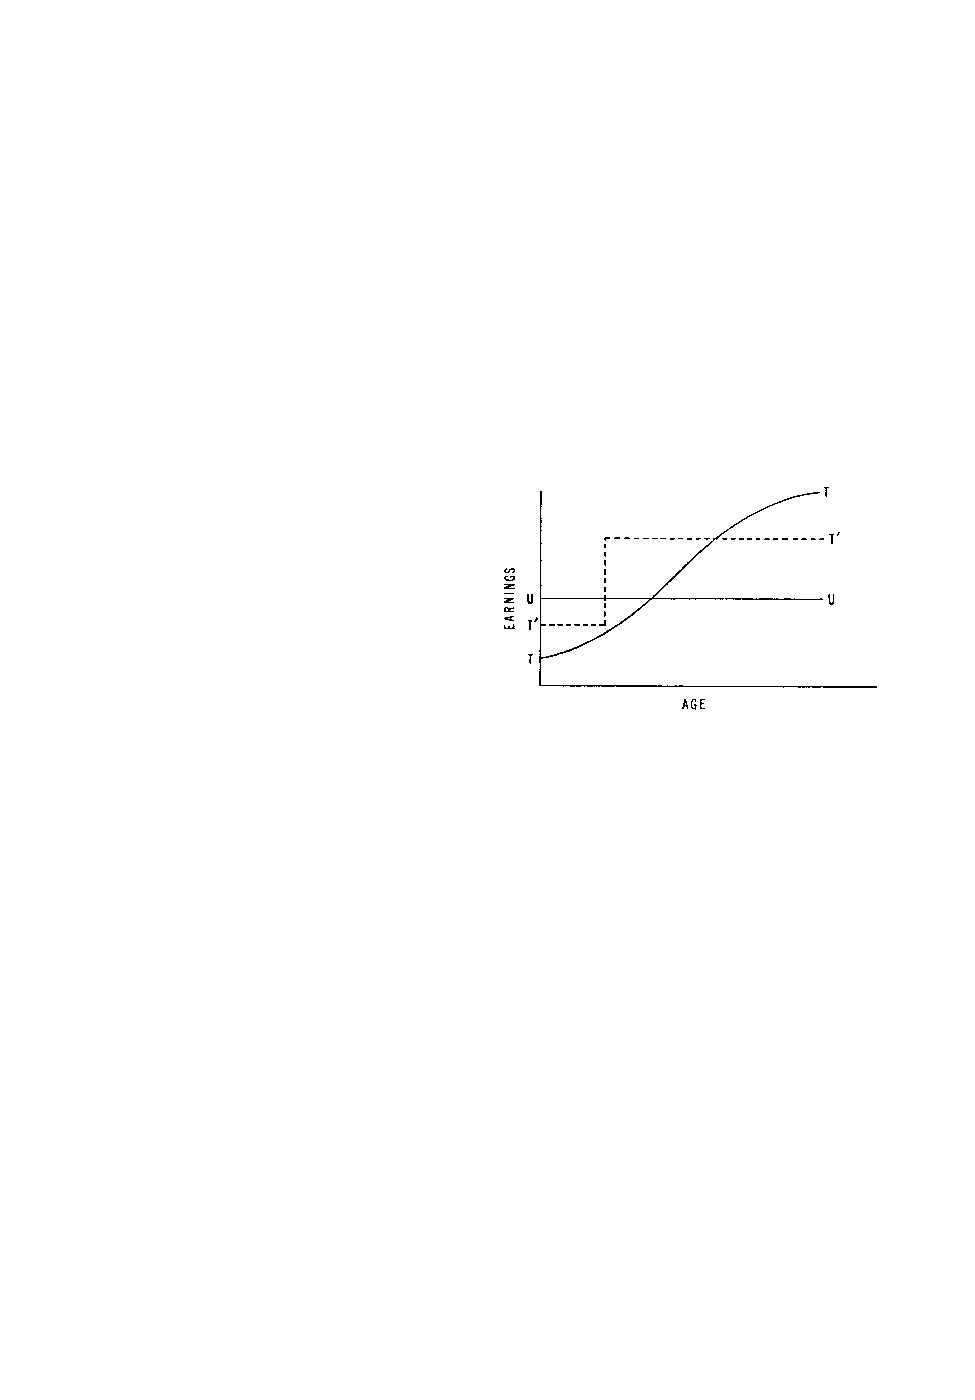
\includegraphics[width=8cm]{fig1.pdf}
        \caption{from Becker, p.15}
        \label{fig1}
      \end{figure}
      UU is the untrained person, TT trained person (first paying for, then collecting rent from training). Difference between UU and TT greater the greater the cost of and return from training. Not only does training make the curve steeper, but also more concave. Extreme case TT'.
    \item Unemployment rates tend to be negatively related to the level of skill
      \begin{itemize}
        \item market demand, $MP$\dots
      \end{itemize}
    \item Firms in underdeveloped countries appear to be more
      "paternalistic" toward employees than those in developed countries
      \begin{itemize}
        \item investment in activities outside the job are done when an
          increase in productivity is the result
        \item e.g. health, anti-alcoholism
        \item thus, this "paternalistic" behavior results from typical
          behavior outside the firm!
      \end{itemize}
    \item Younger persons change jobs more frequently and receive more
      on-the-job training than older persons
      \begin{itemize}
        \item decisions regarding human capital are NPV decisions
        \item therefore, they are driven by the time-frame of the
          decision (on-the-job training)
      \end{itemize}
    \item The distribution of earnings is positively skewed, especially
      among professional and other skilled workers
    \item Abler persons receive more education and other kinds of
      training than others
      \begin{itemize}
        \item higher $MP$...
      \end{itemize}
    \item The division of labour is limited by the extent of the
      market
      \begin{itemize}
        \item a larger market generates \emph{incentives} for more
          specialization, as higher investments in education are
          rewarded by higher wages
        \item thus, a "larger market" implies more demand for
          specialized skills...
      \end{itemize}
    \item the typical investor in human capital is more impetuous and thus
      more likely to err than is the typical investor in tangible capital
  \end{enumerate}
  % section stylized facts (end)

  \subsubsection{Basic Model} % (fold)
  \label{sec:model}
  \begin{eqnarray}
    MP &=& w
  \end{eqnarray}
  Workers have different unique productivities (wages) in each period.
  \begin{eqnarray}
    MP_{t}&=&w_{t}
  \end{eqnarray}
  Training lowers current receipts (R) and raises current expenditures
  (E). However this trend is reversed for future periods. Therefore: NPV
  consideration.
  \begin{eqnarray}
    \sum_{t=0}^{n-1} \dfrac{R_t}{(1+i)^{t+1}} &=& \sum_{t=0}^{n-1}
    \dfrac{E_t}{(1+i)^{t+1}}
  \end{eqnarray}
  Now we only have training in the first period; Expenditures in first
  period are wages + cost of training (k); afterwards only wage. Receipts
  in all periods is MP.
  \begin{eqnarray}
    MP_0 + \sum_{t=0}^{n-1} \dfrac{MP_t}{(1+i)^{t}} &=& W_0 + k +
    \sum_{t=0}^{n-1} \dfrac{W_t}{(1+i)^{t}} \label{eq4}
  \end{eqnarray}
  We define term $G$
  \begin{eqnarray}
    G&=& \sum_{t=1}^{n-1} \dfrac{MP_t - W_t}{(1+i)^{t}}
  \end{eqnarray}
  Now equation (\ref{eq4}) becomes
  \begin{eqnarray}
    MP_0 + G &=& W_0 + k \label{eq6}
  \end{eqnarray}
  Now we need to include the fact that training takes away time from
  production. ($MP'_0$ what could have been produced, $MP_=$ what was
  actually produced, C is the sum of opportunity cost and the outlays on
  training) Equation (\ref{eq6}) becomes
  \begin{eqnarray}
    MP'_0 + G &=& W_0 + C \label{eq7}
  \end{eqnarray}
  We see that G is the excess of future receipts over future outlays (a
  notion of return on training). Optimality condition: $G=C$ (return
  equals cost)
  % section model (end)

  \subsubsection{General Training} % (fold)
  \label{sub:general_training}
  \textbf{General Training:} This kind of training generally increases
  the $MP$ of the worker. Since the worker can switch jobs, he will
  have to bear the costs of this kind of training.

  Hence, $MP$ and $W$ are raised by the same amount! $MP_t = W_t
  \forall t$ 
  \begin{eqnarray}
    G&=& \sum_{t=1}^{n-1} \dfrac{MP_t - W_t}{(1+i)^{t}}=0
  \end{eqnarray}
  Thus, eq. (\ref{eq7}) becomes 
  \begin{eqnarray}
    MP'_0 &=& W_0 +C \\
    \rightarrow W_0 &=& MP'_0 -C
  \end{eqnarray}
  % subsection General Training (end)
  \subsubsection{Specific Training} % (fold)
  \label{sub:Specific_Training}
  \textbf{Specific Training:} This kind of training only increases the
  $MP$ of the worker for the specific firm.
  Consequently, in this extreme case firms are willing to pay for the
  training, since the investment is offset by increases in profit due
  to higher $MP$ of the workers. On the other hand, workers will not
  be willing to invest, since they have "no gain" from this kind of
  investment. The gain is fully absorbed by the firm!
  % subsubsection Specific Training (end)

  \subsection{(Ben-Porath, 1967) "The Production of Human Capital and the Life Cycle of Earnings"} % (fold)
  \subsubsection{Assumptions}
    \begin{enumerate}
      \item Individual utility is not a function of activities involving time as an input.
      \item There is a fixed amount of time to be allocated every period to activities that produce earnings and additions to the stock of human capital.
      \item The stock of human capital, $K$, of which every individual has some initial endowment, is homogeneous and subject to an exogenously given rate of deterioration, $\delta$.
      \item The stock of human capital is not an argument in the individual's utility function.
      \item Unlimited borrowing and lending take place at a constant rate of interest, $r$.
    \end{enumerate}
  \subsubsection{Two stages of decision-making}
  \begin{enumerate}[label={\alph*)}]
      \item The individual allocates the given periods of time between earning and producing human capital and finds the corresponding outlays on investment that maximize the discounted value of any time $t$ of disposable earnings from $t$ to $T$, where $T$ is assumed with certainty to be the end of life.
      \item Given the optimal time path of disposable earnings, the individual decides on the timing of the consumption.
    \end{enumerate}
  \subsubsection{The Model} % (fold)
  \setcounter{equation}{0}
  \begin{itemize}
    \item[$a_0$] wage, or ``rental of human capital''
    \item[$K$] a unit of human capital
    \item[$Y_T$] earning capacity at time $t$
  \end{itemize}

  \begin{align}
    Y_t=\alpha_0K_t
  \end{align}

  \begin{itemize}
    \item[$E_t$] disposable earnings in period $t$
    \item[$I_T$] cost of investment, equal to $(Y_t-E_t)$
  \end{itemize}

  \begin{align}
    \begin{split}
      Q_t&=\beta_0(s_tK_t)^{\beta_1}D^{\beta_2}_t $,$\\
      $where $\beta_1, \beta_2 > 0&$ and $\beta_1+\beta_2<1
    \end{split}
  \end{align}
  \begin{itemize}
    \item[$Q$] flow of human capital produced
    \item[$D$] quantity of purchased inputs
    \item[$P_d$] price of purchased inputs
    \item[$s_t$] fraction of available stock of human capital allocated to the production of human capital
  \end{itemize}
  The fraction $s_t$ is constrained by the condition
  \begin{align}
    0\leqs_t\leq1
  \end{align}
  The rate of change of the capital stock:
  \begin{align}
    \dot{K}_t &= Q_t - \delta K_t
  \end{align}
  \begin{itemize}
    \item[$\delta$] rate by which the stock of human capital deteriorates
  \end{itemize}
  % Decide whether to include any other of the 16 formulas

  \subsubsection{Findings}
  \begin{itemize}
    \item People make most of their investments in themselves when they are young, and to a large extend by foregoing current earnings.
    \item The larger the stock of human capital, the larger the earnings per unit of time that the individual could get in the market and therefore the higher the foregone earnings from diverting a unit of time away from the market.
    \item If $\gamma _{1} = \gamma _{2}$ (Cobb-Douglas: Equation (17), p. 360) the more highly educated person is also better equipped for learning, so that his higher opportunity cost is matched by the greater amount of skills that he can acquire per hour.
    \item If $\gamma _{2} > \gamma _{1}$ capital accumulation reduces the cost of producing human capital, and it is possible even in phase (ii) to have a stretch of time over which investment rises.
    \item Three phases will exist:
      \begin{itemize}
        \item Available stock of human capital $K_t$ is not large enough to satisfy demand.
        \item Available stock is enough to supply the services demanded, so that $0<s<1$ and the services of human capital are truly a variable factor.
        \item Stock of capital is too big so that the optimal policy requires more disinvestment than is feasible through deterioration, that is to produce negative quantities of human capital.
      \end{itemize}
    \item \emph{Normal case}: Capital stock does rise over a period, eventually as gross additions become very small and the stock becomes large this must be reversed, and toward end of life, $T$, the stock will decline, if there is any deterioration.
    \item $\dot{I}$ is always negative. Thus the curve of observed earnings exaggerates the rate of increase of earning capacity when the latter increases and understates its decline when it declines.
    \item If depreciation is zero, there is always, except at point $T$, an increase in the three types of earnings ($E_t$ - disposable earnings, $Y_t$ - earning capacity, $\hat{E}$ - observed earnings), and at each point in time their rank by rate of change will be the reverse of their rank by level.
    \item If there is no deterioration ($\delta = 0$) the ever rising curve of observed earnings is always concave from below.
    \item Possibility that optimal decision requires initial assignment of $s=1$, or $100\%$ of the labour force educating themselves.
  \end{itemize}

  \subsection{(Lazear, 2003) "Firm-Specific Human Capital: A Skill-Weights Approach"} % (fold)
  \subsubsection{Fact sheet} % (fold)
  \begin{enumerate}
    \item The ``skill-weights" view allows skills to be general instead of firm-specific. Instead the relative importance of skills makes them more or less attractive to employers.
    \item $y_i = \lambda_i A+(1-\lambda_i)B$ is the potential earning for a worker with skill set $(A, B)$ at firm $i$.
    \item $\lambda_i$ reflects that firm $i$ may weigh the two skills differently.
    \item $p$ is the probability that the worker is going to stay with the current company in the next period.
    \item The difference between the earnings growth associated with a given amount of experience for those who stay and those who go leads on the \emph{tenure coefficient}. The amount of wage growth the leavers get loads on the experience coefficient.
    \item The worker must chose his investment strategy not knowing whether he will leave the firm or not. $p$ is usually large enough so that he caters to the needs of the first job. When he looses his job he will also loose some income since his skill set will most likely be poorly matched to the new job.
    \item The lower $p$, the less he looses through being let off.
    \item The tenure coefficient should be negatively related to the amount of turnover in the occupation.
    \item Those who leave a firm with unusual weighting patterns suffer larger wage loss for a given $p$.
    \item $Market thickness$ is modeled as allowing more search: Two draws occur, for the second of which the worker can decide whether to switch jobs or not.
    \item In thicker markets a worker looses less on a move despite a more idiosyncratic investment strategy.
    \item Investment increases over time because except for a perfect match between the preferences of the first and second company another round of investment is appropriate.
    \item It is possible to generate tenure coefficients that are nearly the same size as the experience coefficients ($90\%$).
    \item The higher $p$, the large the tenure coefficient.
    \item When $\lambda$ takes extreme values it tends to be far away from $\bar{\lambda}$, which is why the uniform distribution yields lower tenure coefficients than the bimodal.
  \end{enumerate}

  \subsubsection{Findings}

    The tenure effects found in the empirical literature do not fit examples of firm-specific human capital well. The proposed approach of weighted general human capital provides the same implications but is more realistic.
    \begin{itemize}
      \item Like the traditional view, the skill-weights approach implies that workers who experience an exogenous change in job lose some earnings associated with their previous tenure
        \begin{itemize}
          \item Loss grows as workers are with firm for longer.
          \item Loss tends to be greatest when employment most secure.
          \item The more idiosyncratic the firm's technology the larger is the loss.
          \item Workers hedge against this loss by adopting a more external- oriented investment strategy.
        \end{itemize}
      \item Size of the tenure coefficient varies with the thickness of the market.
      \item A firm may bear some or even most of the cost of skills that look general.
    \end{itemize}

  \section{Meeting 4: Informal Learning} % (fold)
  \label{prt:Meeting 4}
  \subsection{(Destré et al., 2006) "Learning form experience or learning from others?"} % (fold)
  \label{sec:Destre2006}
  \setcounter{equation}{0}
  \subsubsection{Introduction} % (fold)
  \label{ssub:Introduction}
  \begin{itemize}
    \item Mincerian earnings function: Linear in education, quadratic in labor market experience.
    \item extended version: includes a quadratic function of tenure in the incumbent firm
  \end{itemize}
  Here, the authors have a dataset based in France, of 150,000 wage earners and 16,000
  establishments. They furthermore distinguish informal training by means of learning from own
  experience and learning from others.
  
  \begin{figure}[ht]
        \centering
        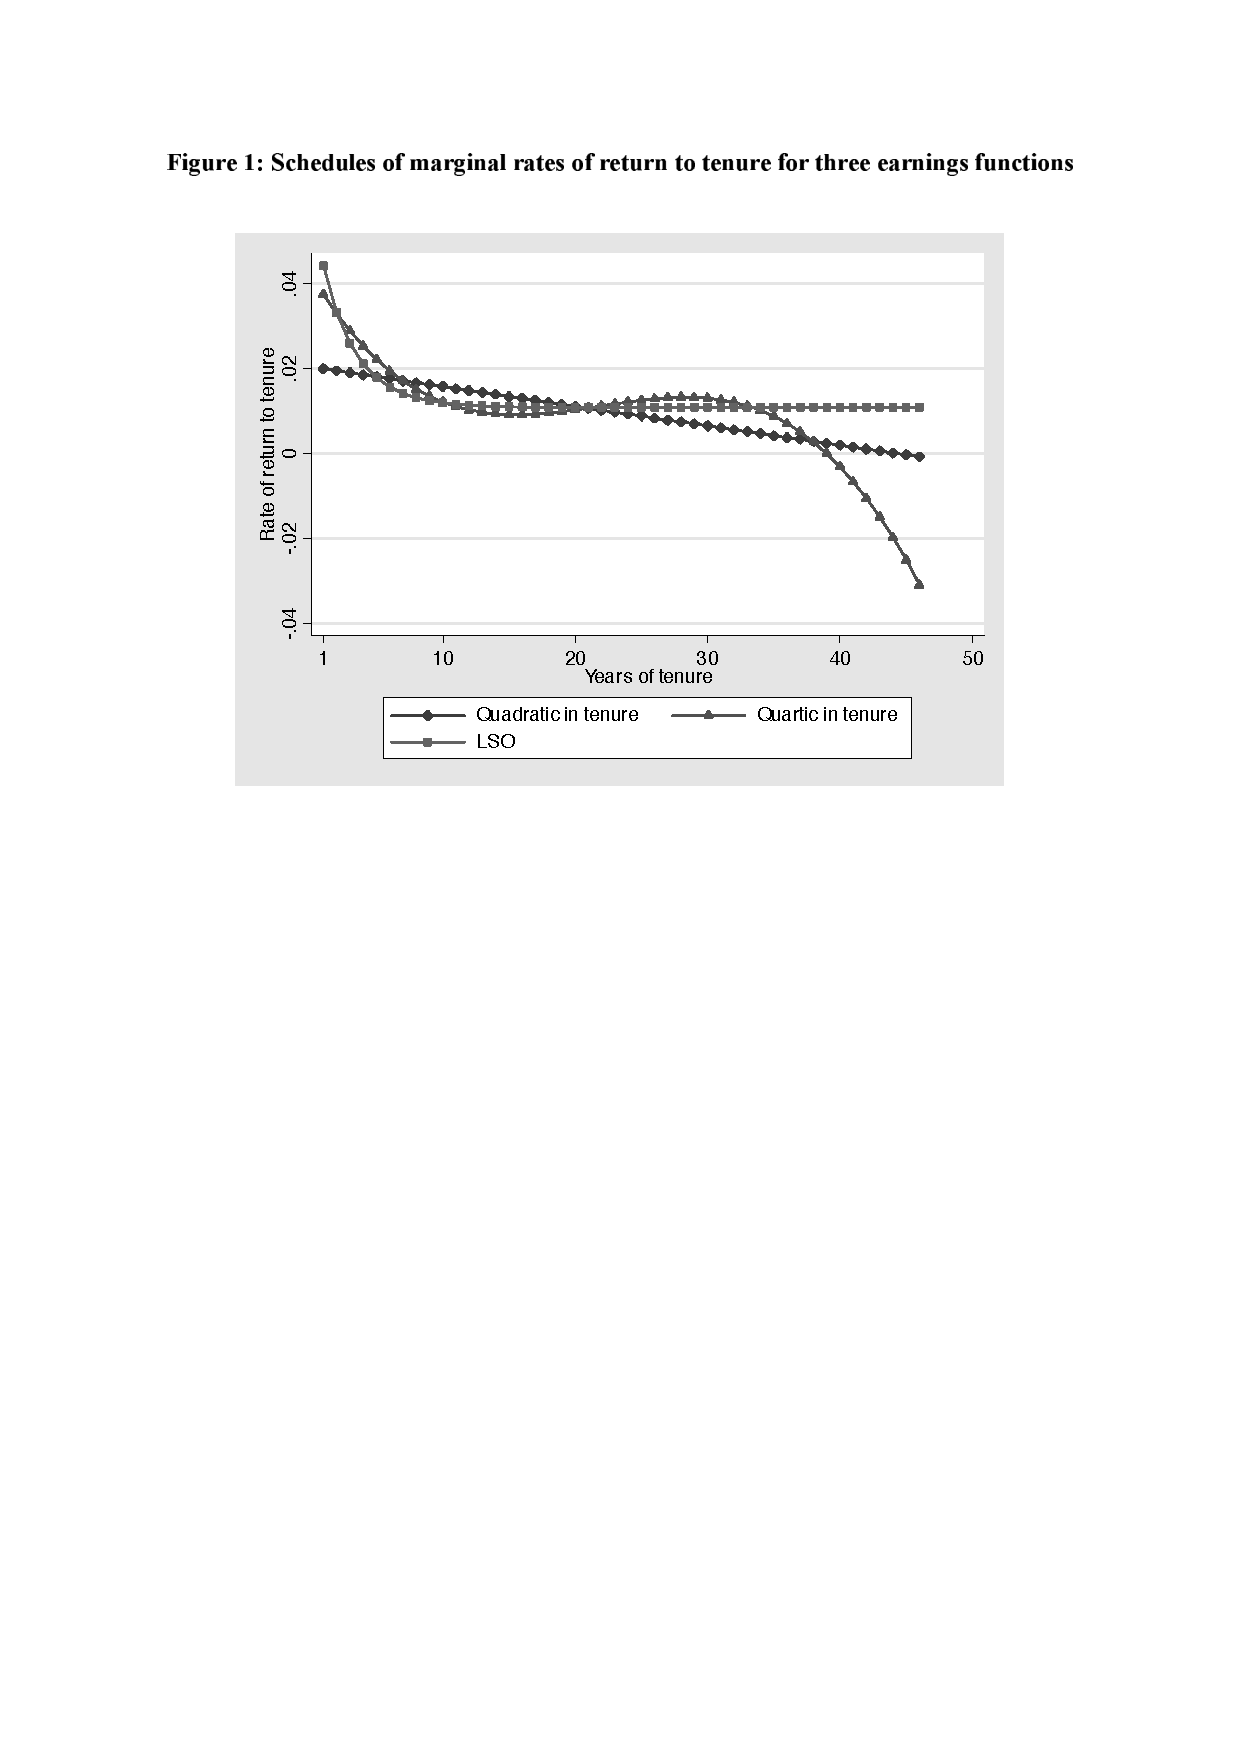
\includegraphics[width=12cm]{dest_1.pdf}
        \caption{Destre, p. 30}
        \label{dest_1}
  \end{figure}


  % TODO decide whether the illustration make sense to include
  % TODO position them in the summary
  % TODO reference them in the text, explain if necessary
  \subsubsection{Illustrations to be included. …or not.}
    \begin{figure}[htb]
      \centering
      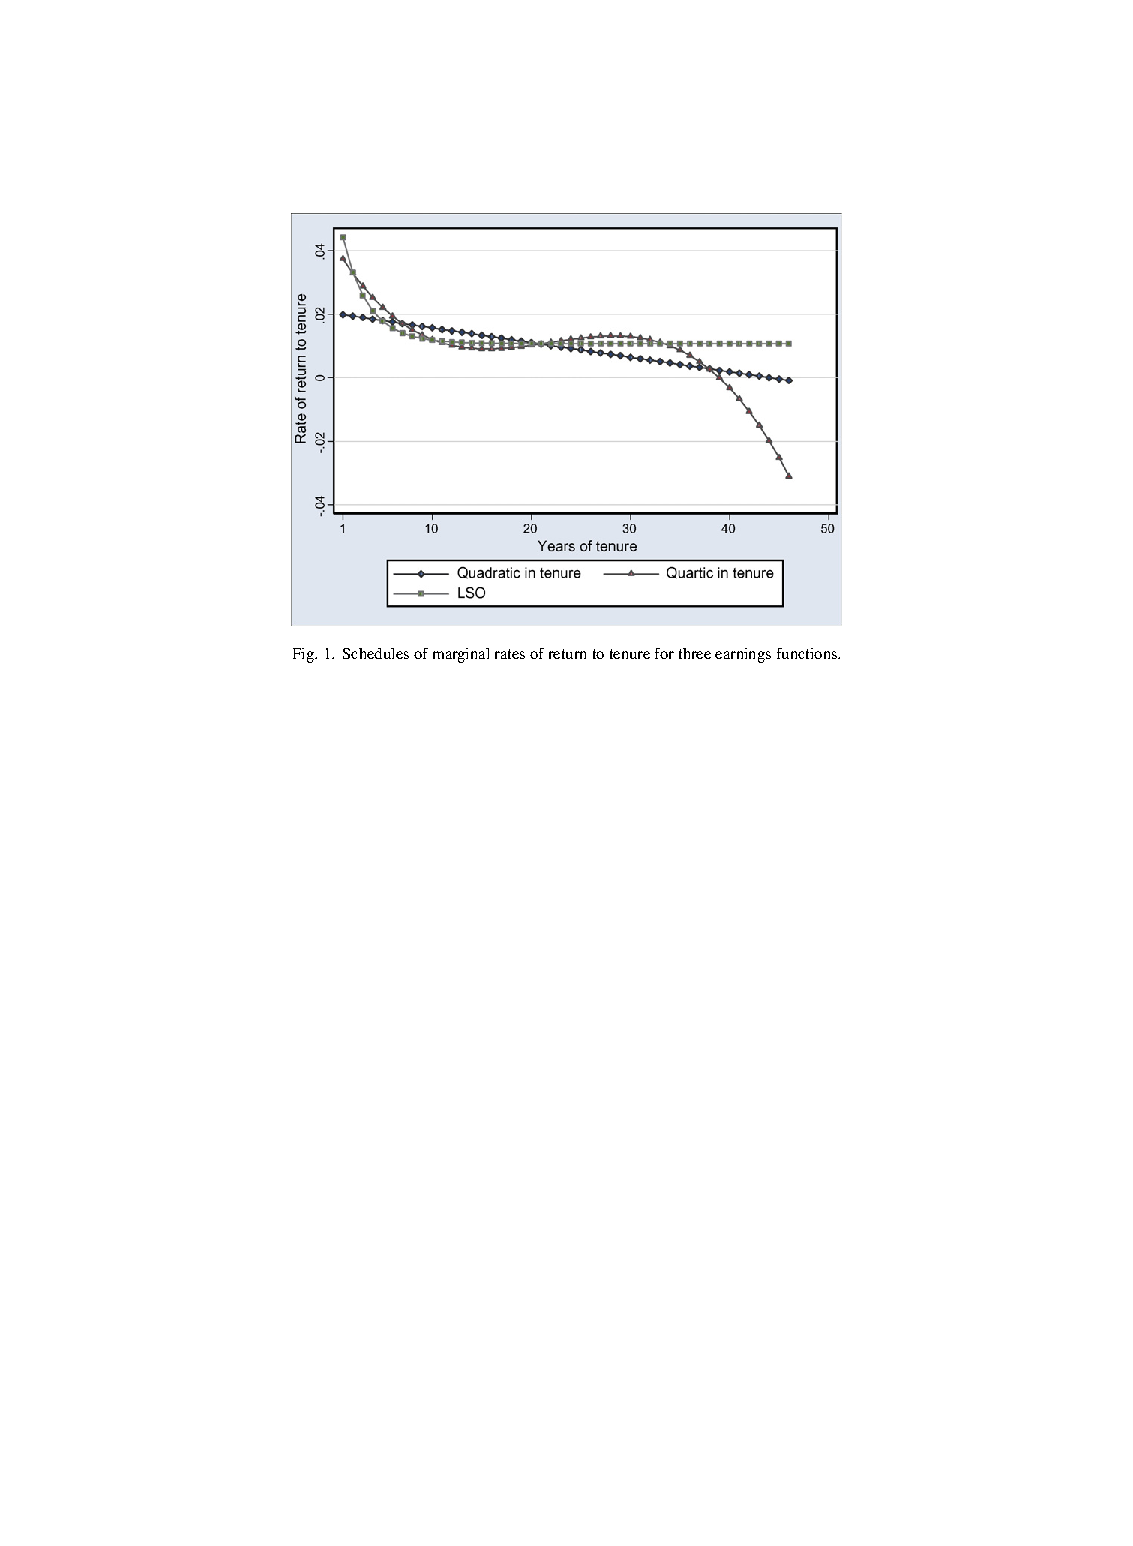
\includegraphics[width=12cm]{Meeting 4 LEARNING FROM EXPERIENCE - Seite 932.pdf}
      \caption{Destré et al., p. 935: "Schedules of marginal rates of return to tenure for three earnings functions" see also section~\ref{sec:Destre2006}}
      \label{fig:Destré marginalreturntotenureearningfunction}
    \end{figure}


    \begin{figure}[htb]
      \centering
      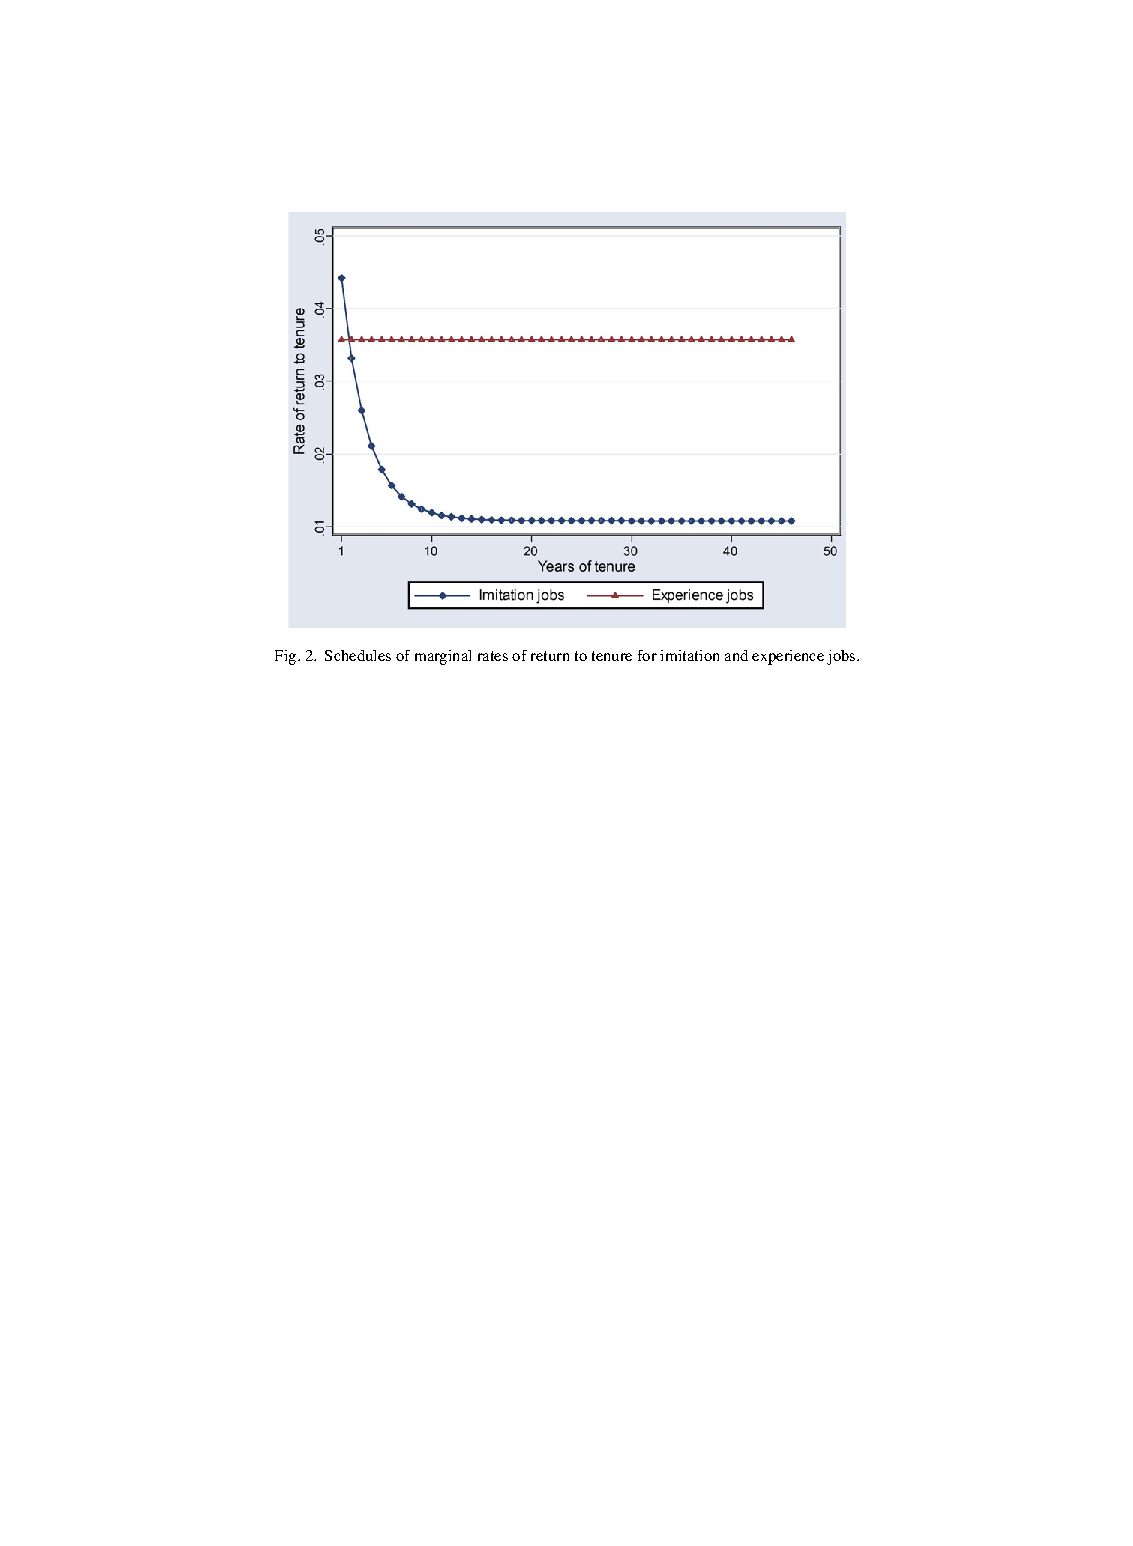
\includegraphics[width=12cm]{Meeting 4 LEARNING FROM EXPERIENCE - Seite 935.pdf}
      \caption{Destré et al., p. 935: "Schedules of marginal rates of return to tenure for imitation and experience jobs" see also section~\ref{sec:Destre2006}}
      \label{fig:Destré marginalreturntotenure}
    \end{figure}




  \subsubsection{Informal learning on-the-job from self and others: theory} % (fold)
  \label{ssub:Informal learning on-the-job from self and others: theory}
  \begin{itemize}
    \item workers acquire job-specific training, either formally or informally. Both forms are
      costly, but the difference is that purely informal learning does not take time away from
      others.
    \item informal training often depends on the work contract. workers are "forced" to acquire the
      knowledge of the firm. Thus, workers bear the cost of training, but also reap the rewards.
  \end{itemize}
  Formally, for worker $i$ in firm and job $j$ and time period $t$: Job-specific human capital
  $h_{ijt}$. $H_{ijt}$ is the human capital level of the "teacher" for informal learning. Factor
  $g$ is the depreciation rate of human capital (normally positive). $n$ is the rate of knowledge
  diffusion in the firm.
  \begin{eqnarray}
    h_{ijt}- h_{ij,t-1} &=& gh_{ij,t-1}+ \dfrac{n}{1+n}(H_{ij,t-1} - h_{ij,t-1} ), \forall t \geq
    1
  \end{eqnarray}
  Furthermore, it is shown how job-specific human capital grows with "tenure" (time on the job).
  \setcounter{equation}{2}
  \begin{eqnarray}
    h_{ijt} &=& (1+g)^t h_{ij0} (1+(k^t)\lambda_{ij}) , \mbox{  with  } \lambda_{ij} =
    \dfrac{H_{ij0}}{h_{ij0}} -1 \forall \lambda{ij} \geq 0
  \end{eqnarray}
  $\lambda_{ij}$ denotes the job-specific learning from others' potential, it is independent of
  tenure. Now, the equation is converted in natural logarithms (for econometric estimation)
  \begin{eqnarray}
    \log h_{iht} &=& \log h_{ij0} + gt + \log (1+ \lambda_{ij}(1-k^t))
  \end{eqnarray}
  $\lambda$ can probably be approximated:
  \begin{eqnarray}
    \log h_{iht} &=& \log h_{ij0} + gt + \lambda_{ij}(1-k^t) \mbox{  with  } \lambda_{ij} = \log
    \dfrac{H_{ij0}}{h_{ij0}}
  \end{eqnarray}
  Now, the logarithm of gross earnings is the sum of a linear-in-tenure experience effect and an
  exponential effect of learning from others that converges fast towards the firm's job-specific
  learning potential.

  \subsubsection{The returns to tenure} % (fold)
  \label{ssub:The returns to tenure}
  The marginal returns to tenure ($R$) are defined as:
  \begin{eqnarray*}
    R_{ijt} &=& \dfrac{h_{ijt}- h_{ij,t-1}}{h_{ij,t-1}} \mbox{  } \forall t \geq 1
  \end{eqnarray*}
  "after a few manipulations"
  \begin{eqnarray}
    R_{ijt} &=& g + \dfrac{n}{n+1} \left( \dfrac{\lambda_{ij} k^{t-1}}{1+\lambda_{ij}(1-k^{t-1})} \right)
  \end{eqnarray}
  \begin{itemize}
    \item returns to tenure is from dependent
    \item also depends on teacher/worker knowledge ratio
    \item marginal returns to tenure are shown to be a concave increasing function of the
      job-specific learning potential
    \item there is also a convex decreasing relation of the marginal return to tenure with tenure
    \item increasing the efficiency of learning from others on-the-job will benefit low-tenured
      workers who will learn faster, but it will reduce what remains to be learned from others in
      the future
  \end{itemize}
  \begin{eqnarray*}
    \dfrac{\delta R_{ijt}}{\delta g} & \geq & 1, \mbox{  for  } t \geq 2 \mbox{  and  }
    \lambda_{ij} \geq 0 \mbox{  } (=1 \mbox{  if  } \lambda_{ij}=0)
  \end{eqnarray*}
  Increasing the efficiency of experience initially increases the self-learning effect but this will
  provoke a multiplier effect in subsequent periods by raising the firm's knowledge.
  % subsubsection The returns to tenure (end)

  \subsubsection{Data and econometric specification} % (fold)
  \label{ssub:Data and econometric specification}
  Large French cross section with matched employer-employee data, 1992 INSEE survey on labor cost
  and wage structure. Carried out across all EU countries. Regression analysis... additional
  variables defined in table 1 (p. 926).
  % subsubsection Data end econometric specification (end)

  \subsubsection{Informal learning on-the-job from self and others: results} % (fold)
  \label{ssub:Informal learning on-the-job from self and others: results}
  Summary of the results is given in table 2 (p. 929). Core yelling points:
  \begin{itemize}
    \item on average, it takes 1.93 years for a worker to embody 50\% of what she can learn from
      others in her establishment, and 9.37 years to embody 95\% of this in total
    \item in contrast to the mincerian model, the return on education is slightly lower, this is
      because one can "learn less" in the firm (regarding return on tenure!)
    \item less educated workers typically make up for lower education by more work-based learning
  \end{itemize}
  % subsubsection Informal learning on-the-job from self and others: results (end)

  \subsubsection{firm's knowledge and the returns to tenure} % (fold)
  \label{ssub:firm's knowledge and the returns to tenure}
  In terms of core yelling points: if there is more knowledge in the firm, the worker will have
  (depending on the functional form that is specified in the model) a generally higher return on
  tenure, since he will be able to learn more!
  % subsubsection firm's knowledge and the returns to tenure (end)


  \subsubsection{job heterogeneity} % (fold)
  \label{ssub:job heterogeneity}
  The teacher/worker knowledge ratio is quite different per firm. They then divide jobs in two
  categories, imitation jobs and experience jobs. Jobs that have a low potential to learn from
  others are called experience jobs. When you can learn from others: Imitation job. Majority of jobs
  are imitation jobs, only 15.8\% of jobs are classified as experience jobs. Return on tenure and
  t/w ratio differ for these jobs!  See table 6 (p. 933).
  % subsubsection job heterogeneity (end)

  \subsubsection{dualism at the establishment's level} % (fold)
  \label{ssub:dualism at the establishment's level}
  (Establishment: Employer) ... same conclusions can be drawn ...
  % subsubsection dualism at the establishment's level (end)

  \subsubsection{learning from jobs or learning from firms?} % (fold)
  \label{ssub:learning from jobs or learning from firms?}
  See figure 2 (p. 935), the rate of return to tenure is strongly decreasing for imitation jobs,
  whereas it stays constant for experience jobs! Furthermore, the average marginal rate of return to
  self-learning is considerably higher for experience jobs than for imitation jobs. Workers with
  experience jobs don't learn from others but by themselves. The marginal returns to education are
  lower in imitation jobs, more educated workers have less to learn from others.
  % subsubsection learning from jobs or learning from firms? (end)

  \subsubsection{conclusions} % (fold)
  \label{ssub:conclusions}
  The authors have suggested a simple model of informal learning on-the-job
  which combines learning from (own) experience and learning from others.  They
  find that workers on average can learn from others 10\% of their own human
  capital on entering the firm, and catch half of their learning potential in
  just 2 years. Since individuals learn fast from their co-workers, the
  estimated returns to tenure loom larger than predicted by a quadratic, or
  even a quartic-in-tenure, Mincerian function in the first years and decline
  more sharply (until about 30 years). Learning by watching accounts for three
  quarters of the marginal rate of return in the first year of tenure, but this
  share falls rapidly, with an average of 12\%. While education and
  self-learning on-the-job are complementary, education and learning from
  others on-the-job are substitutes. The more education, the less can be
  learned from others.\\
  This forces the private marginal return curve to decline with education, an
  effect which was not captured by current theory.  Seen from a different
  perspective, the more educated workers share the social returns of their own
  education with their less qualified co-workers.  The potential for learning
  from others on the job varies across jobs and establishments, and this
  provides a new distinction between imitation jobs and experience jobs.
  Workers in imitation jobs, who learn most from others, tend to have
  considerably longer tenure than workers in experience jobs.\\
  The latter are more mobile and have accumulated more market experience.
  Although workers in experience jobs can learn little from others, we find
  that they learn a lot by themselves. Consequently, we do not find a close
  correspondence between the imitation jobs/experience jobs “dualism” and the
  primary/secondary jobs and firms’ dualism implied by the dual labor market
  theory. Even though imitation jobs imply far less turnover than experience
  jobs, imitation jobs do not appear to be “better” in terms of education
  levels and wages. We show, however, that predictions of the dual labor market
  theory which cannot be observed at the job’s level under our classification
  of jobs emerge from the aggregation of jobs at the establishment level. 
  % subsubsection conclusions (end)

  \subsection{(Ertaut, 2000) "Non-formal learning and tacit knowledge in professional work"} % (fold)
  \label{sec:Ertaut2000}

  % TODO decide whether the illustration make sense to include
  % TODO position them in the summary
  % TODO reference them in the text, explain if necessary
  \subsubsection{Illustrations to be included. …or not.}

    \begin{figure}[htb]
      \centering
      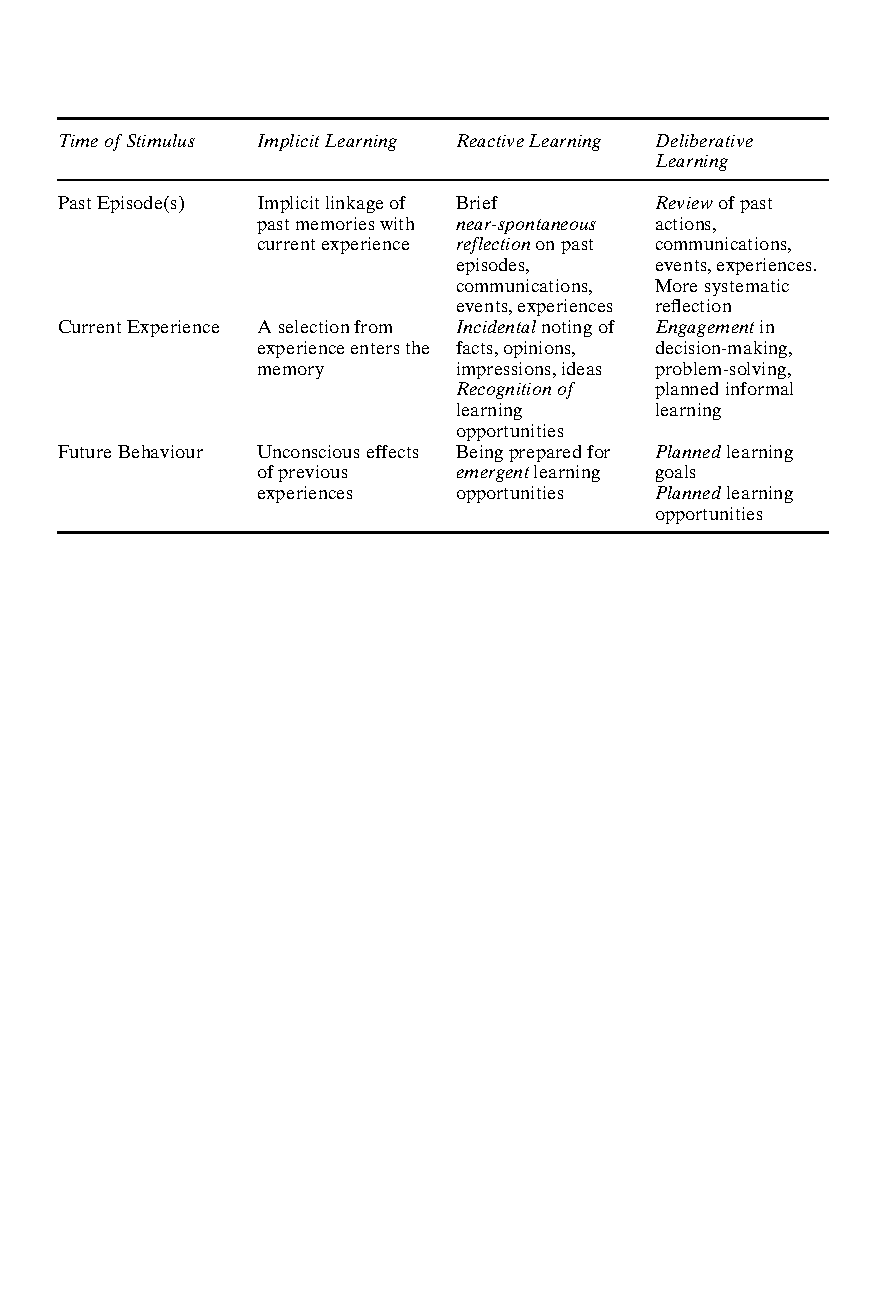
\includegraphics[width=12cm]{Meeting 4 NON-FORMAL LEARNING - Seite 4.pdf}
      \caption{Ertaut, p. 4: "A typology of non-formal learning" see also section~\ref{sec:Ertaut2000}}
      \label{fig:Ertaut typology}
    \end{figure}


    \begin{figure}[htb]
      \centering
      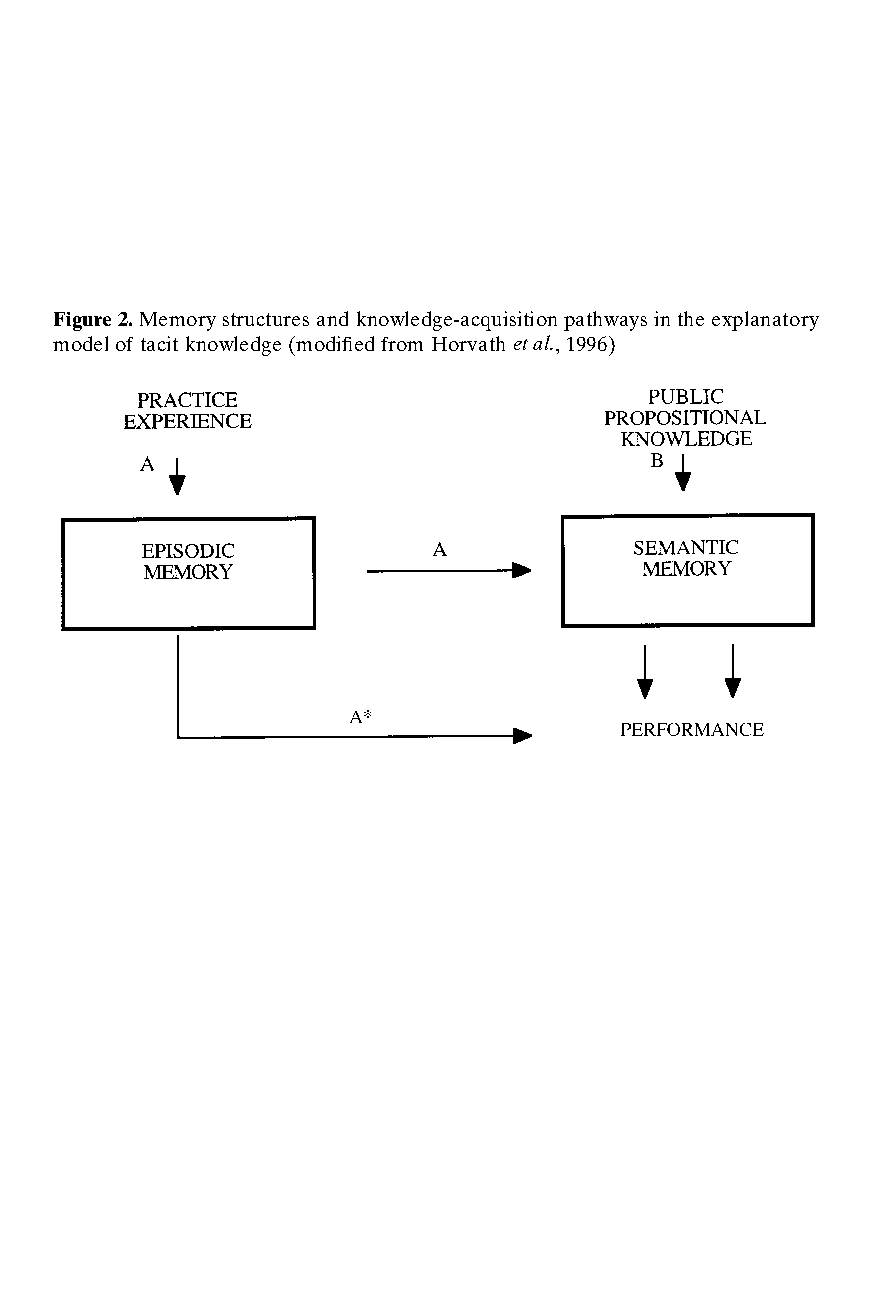
\includegraphics[width=12cm]{Meeting 4 NON-FORMAL LEARNING - Seite 5.pdf}
      \caption{Ertaut, p. 5: "Memory structures and knowledge-acquisition pathways in the explanatory model of tacit knowledge" see also section~\ref{sec:Ertaut2000}}
      \label{fig:Ertaut tacitknowledgemodel}
    \end{figure}



    \begin{figure}[htb]
      \centering
      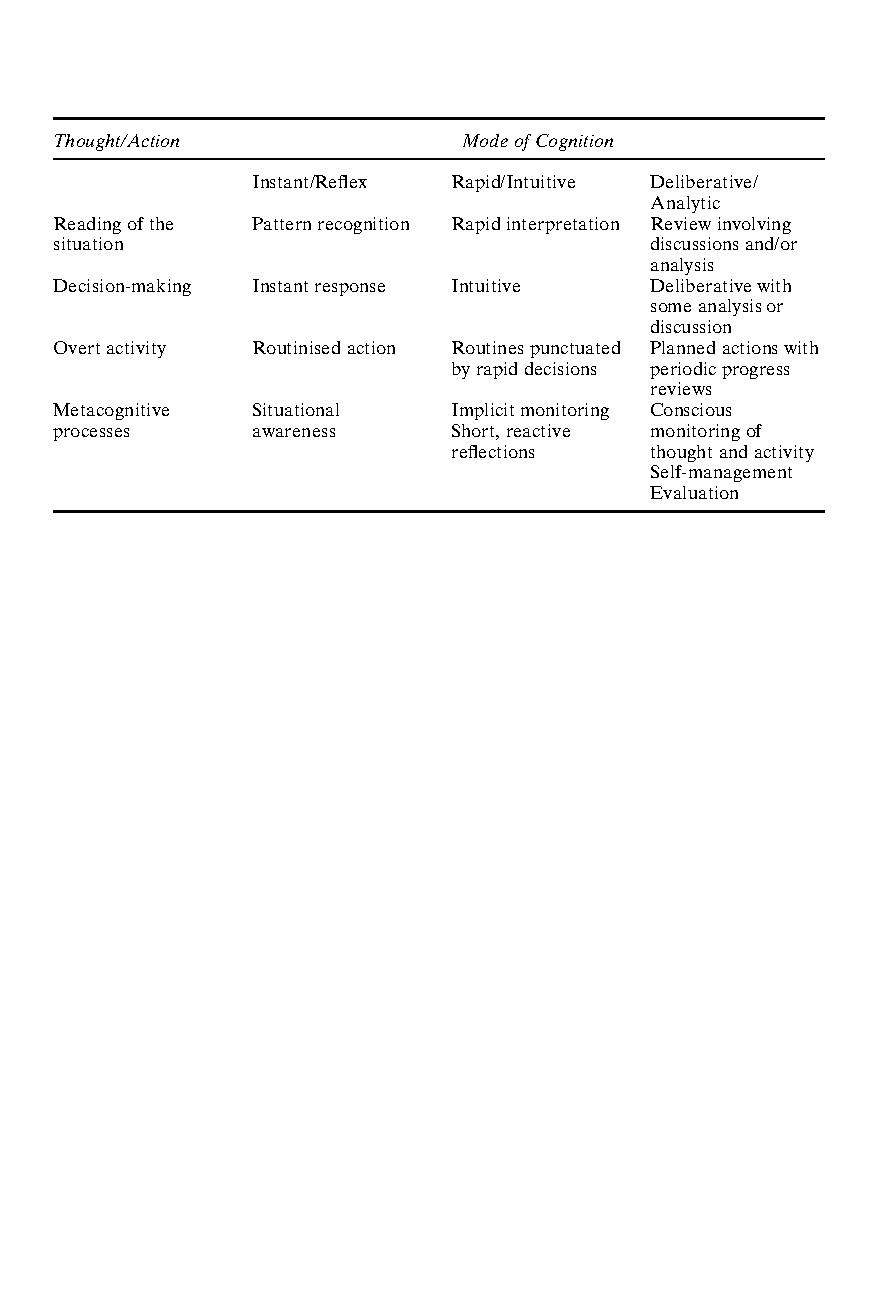
\includegraphics[width=12cm]{Meeting 4 NON-FORMAL LEARNING - Seite 17.pdf}
      \caption{Ertaut, p. 17: "Interactions between time, mode of cognition and type of thought/action" see also section~\ref{sec:Ertaut2000}}
      \label{fig:Ertaut cognitioninteractions}
    \end{figure}



    \subsubsection{Approach}
      Exploration of professional education and learning in the workplace. The aim is the clarification of the terminology associated with \emph{non-formal learning}, \emph{implicit learning} and \emph{tacit knowledge}. Discussion of implications of these concepts to professional practice.

    \subsubsection{Definitions}
      \textsc{non-formal learning}: distinguishes between \emph{implicit learning}, \emph{reactive on-the-spot learning} and \emph{deliberative learning}. \\
      \textsc{tacit knowledge}: \emph{tacit understanding} of people and situations, \emph{routinised actions} and the \emph{tacit rules} that underpin intuitive decision-making. They come together when professional performance involves sequences of routinised action punctuated by rapid intuitive decisions based on tacit understanding of the situation. \\
      \textsc{tacit processes}: \emph{reading the situation}, \emph{making decisions}, \emph{overt activity} and \emph{metacognition}.\\
      \textsc{modes of cognition}: \emph{intuitive}, \emph{analytic} and \emph{deliberative}. The balance between these modes depends on time, expericen and complexity.Where rapid action dominates, periods of deliberation are needed to maintain critical control.
    \subsubsection{Findings}
      Types of situation in which \emph{tacit knowledge} is acquired or used:
      \begin{itemize}
        \item Knowledge acquired by \emph{unaware implicit learning}
        \item Knowledge \emph{inferred by observers} such as implicit theories of action, schemas
        \item Knowledge which enables \emph{rapid, intuitive understanding} and \emph{response}
        \item Knowledge entailed in \emph{transferring} knowledge \emph{from one situation to another}
        \item Knowledge embedded in \emph{taken-for-granted activities}, \emph{perceptions} and \emph{norms}
      \end{itemize}
      \\
      Tacit knowledge may be made specific and this is desirable in order to
      \begin{itemize}
        \item improve quality or \emph{performance} of a person or a team
        \item help \emph{communicate} knowledge to another person
        \item \emph{link} aspects of performance with desirable outcomes
        \item construct artifacts to \emph{assist decision-making} or reasoning
      \end{itemize}
      Improvement of performance is dependent on feedback. Tacit knowledge which may lie behind an action can be problematic to communicate as there is a difficulty in explaining perceptions. An observer has no access to the performer's thoughts or knowledge base. Explicitness is needed for improving performance and accountability.


  % section (Ertaut, 2000 (end)
  % part Meeting 4 (end)

\section{Meeting 5: Selection Bias in Return on Education} % (fold)
\label{sec:Meeting 5}
  \subsection{(Leuven \& Oosterbeek, 2008) "An alternative approach to estimate the wage returns to private-sector training"} % (fold)
  \label{sub:}
  This paper introduces the two typical kinds of upward biases found in the studies on return on education / private-sector training. These biases
  are the selection bias and the bias of unobservables. ($\rightarrow$ ability bias)
  \begin{itemize}
    \item There is a selection bias in many regressions of wages on training, since more able workers (= higher productivity and higher wages) self-select into training.
    \item It is also hard to find variables that only affect training, but not wages (this is called bias of unobservables)
    \item Thus, the effect of private-sector training is typically overstated
    \item In this paper, the authors compare the effect of private-sector training on wages of workers that took training to workers who \textbf{wanted} to take training, and to workers
          who wanted to take training but could not do so due to some random event. (Such as illness, etc.)
    \item Here, the selection bias should be much smaller, because the comparison group \textbf{self-selected} into pursuing training
          but could not attend. 
  \end{itemize}
  Using the technique described above, the authors find a return on private-sector training of 9.5\% (using simple OLS). 
  However, comparing those workers who wanted to participate but did not with those who actually participated yields a
  smaller return: 6.3\%. The comparison group of workers who wanted to attend but couldn't is too small to make any
  statements that are statistically significant.
  % subsection  (end)
  \subsection{(Leigh, 2008) "Estimating returns to education using different natural experimentation techniques"} % (fold)
  \label{sub:leigh}
  The authors try to find the return on education in Australia using three natural experiments. Using a regular
  OLS regression, the return on one additional year of schooling is estimated to be 12\%. However, taking
  the natural experiments into account:
  \begin{enumerate}
    \item \textbf{Month of birth}\\
          Here they look at individuals that are born just one month to late to begin schooling with their cohort.
          Because they assume that the other characteristics are comparable, they can identify the return (in terms of wages)
          of one more year of schooling.\\
          The estimated return on one additional year of schooling is found to be 8\%, which in comparison with the OLS
          estimate suggests an ability bias of about 30\%.
    \item \textbf{Changes in compulsory schooling laws}\\
          Here they look at years in which the number of years of schooling was changed in the legislature.
          Therefore the authors again have a basis of comparison, because again most other characteristics of the
          observations are likely to be the same.\\
          The estimated return on one additional year of schooling is found to be 12\%
    \item \textbf{Twins}\\
          Here they look at wage differences between twins that have obtained different levels of education.
          Because the twins are genetically (nearly) identical, they share most of the other characteristics
          apart from schooling. The authors use this method to confirm their findings (OLS, IV birth, IV law).
          However, the results are somewhat ambiguous.
  \end{enumerate}
  % subsection leigh (end)
  \subsection{(Bedi \& Gaston, 1999) "Using variation in schooling availability to estimate educational returns for Honduras"} % (fold)
  \label{sub:bedi}
  The authors estimate the return on schooling in Honduras (for males) by looking at the actual availability of schools at the
  time when the individuals were eligible to start schooling. It is pointed out that most studies so far only concentrate
  on developed countries.\\
  By adding school availability as an instrumental variable (see appendix~\ref{IV}), the authors estimate the return
  on schooling to be higher than in a standard OLS regression (based on developed countries). Another interesting effect
  that is mentioned by the authors is that individuals with a low marginal return on schooling are more likely to
  be affected by low school availability. Thus, those individuals that are per se less likely to attend school will
  be thwarted away. Therefore, the low availability of schools hits "the lower end of the social spectrum" hardest.\\
  Furthermore, the authors provide insights that show higher returns on schooling, when schools are scarce. In most
  studies the availability of schools is taken as granted, thereby negating the endogeneity of education.\\
  
  % subsection bedi (end)
  \subsection{Takeaway} % (fold)
    \begin{itemize}
      \item self-selection of clever people: overestimation of the effect of education $\rightarrow$
        bias
      \item unobserved factors; ability versus cost of education
      \item policy implications: Honduras, worthwhile to invest in education? / Which level of
        education?
      \item when access to schools is not abundant, the return on schooling is higher.
      \item the return on schooling / training is typically between 5 - 10 \%
    \end{itemize}
    % subsection General Remarks (end)
% section Meeting 5 (end)
  
  \section{Meeting 7: Measuring Skills} % (fold)
  \label{sec:Meeting 7}
    \subsection{(Tomlinson, 1997) "Measuring competence and knowledge using employee surveys: evidence using the British Skills Survey of 1997"}
    \label{sec:Tomlinson1997}


  % TODO decide whether the illustration make sense to include
  % TODO position them in the summary
  % TODO reference them in the text, explain if necessary
  \subsubsection{Illustrations to be included. …or not.}
    \begin{figure}[htb]
      \centering
      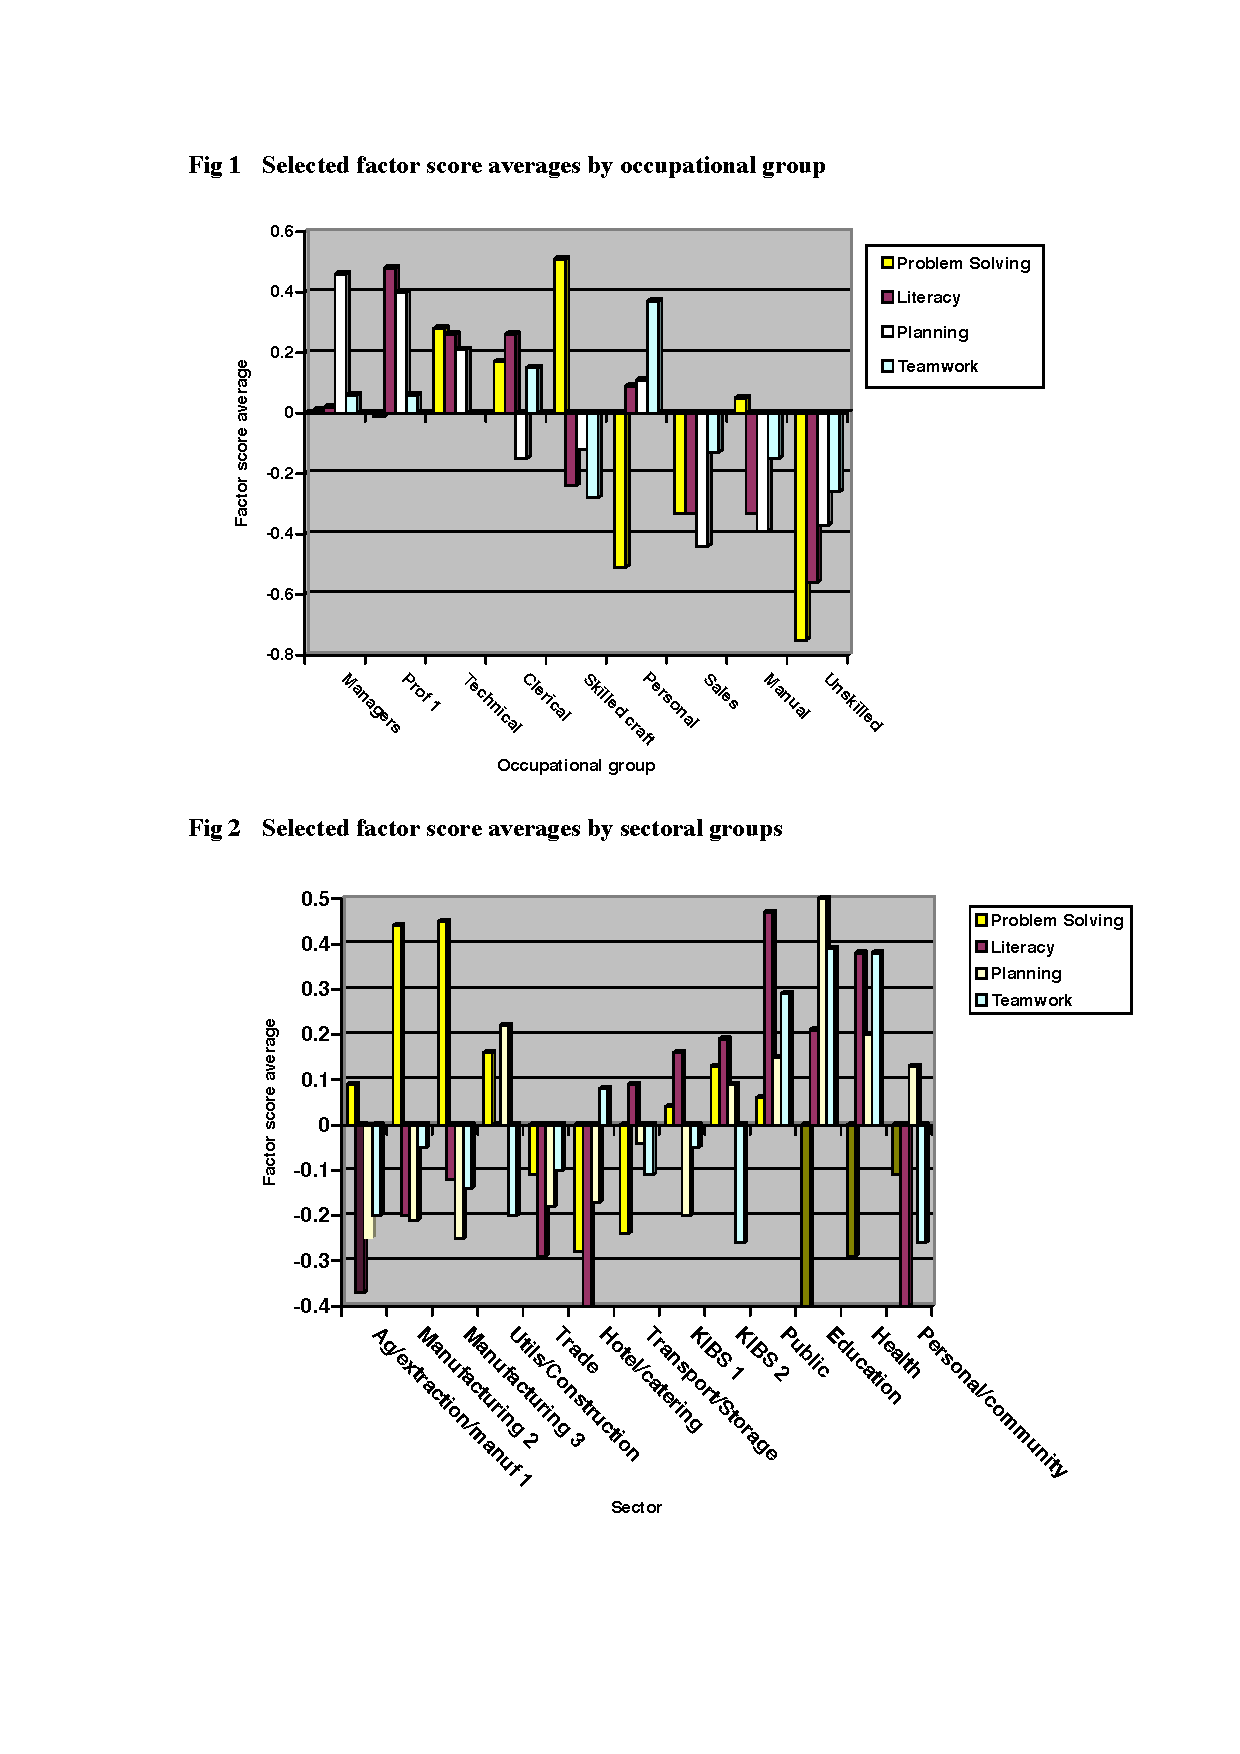
\includegraphics[width=\textwidth]{Meeting 7 dp50 - Seite 15.pdf}
      \caption{Tomlinson, p. 15: "Selected factor score averages by occupational and sectorial groups" see also section~\ref{sec:Tomlinson1997}}
      \label{fig:Tomlinson factorscores}
    \end{figure}

      \subsubsection{Approach}
        Measuring learning in the UK and relate this to competence building systems. Get to grips with the learning economy and the role of knowledge in economic systems, draw conclusions about public policies. Uses the British Skills Survey (bss.dta, 1997) which contains self-assessment on a wide range of skills.

      \subsubsection{Findings}
        The demonstrated micro approach to knowledge and competence measurement using employee level data is a useful complement to macro-level analysis. Certain groups of workers are well ahead in the learning and knowledge stakes, mostly comprised of managers and professional workers. There are sectoral differences, for example manufacturing is predominated by advanced problem solving skills. Services on the other hand are associated with literacy, planning and teamwork skills. High technology sectors are the only ones showing significant gains over others.

        The impact of introduction of computerised equipment was pervasive, affecting all dimensions of knowledge. Results suggest that there are still significant gains to be made from the use of computers. Even moderate use of computers appeared to lead to significant gains in all eight competences.

        Also certain management and workplace practices have a significant impact on learning and competence building. Especially communications within the firm are significant, such as meetings where views can be expressed, quality circles and team based working. Job mobility within firms led to faster learning than job mobility between firms. A surprising result: The relative lack of impact of social relations with fellow workers.

  % section Meeting 7 (end)

  \section{Meeting 8: Depreciation of Skills} % (fold)
  \label{sec:Meeting 8}
  \subsection{(De Grip \& Van Loo, 2002) "The Economics of Skills Obsolescence: A Review"} % (fold)
  \label{sub:grip}
  The authors summarize the literature on skills obsolescence. Three main types are identified (see figure~\ref{skill_obs}).
  \begin{itemize}
    \item  \textbf{Technical Skills Obsolescence}\\
    This type captures the depreciation of human capital that takes place either through the ageing process
    (or illness, injury) or through atrophy (the skill is not used and this forgotten). Atrophy is an interesting factor here,
    because the effect is very pronounced during unemployment, when most of the skills of an individual are just not used. The
    chapter mentions a study about the "age-earning profile in case of work interruption". This study does not only take unemployment
    into consideration, but mostly women giving birth, or cases of prolonged sickness. (see figure~\ref{age_earn})

    \begin{figure}[htb]
      \centering
      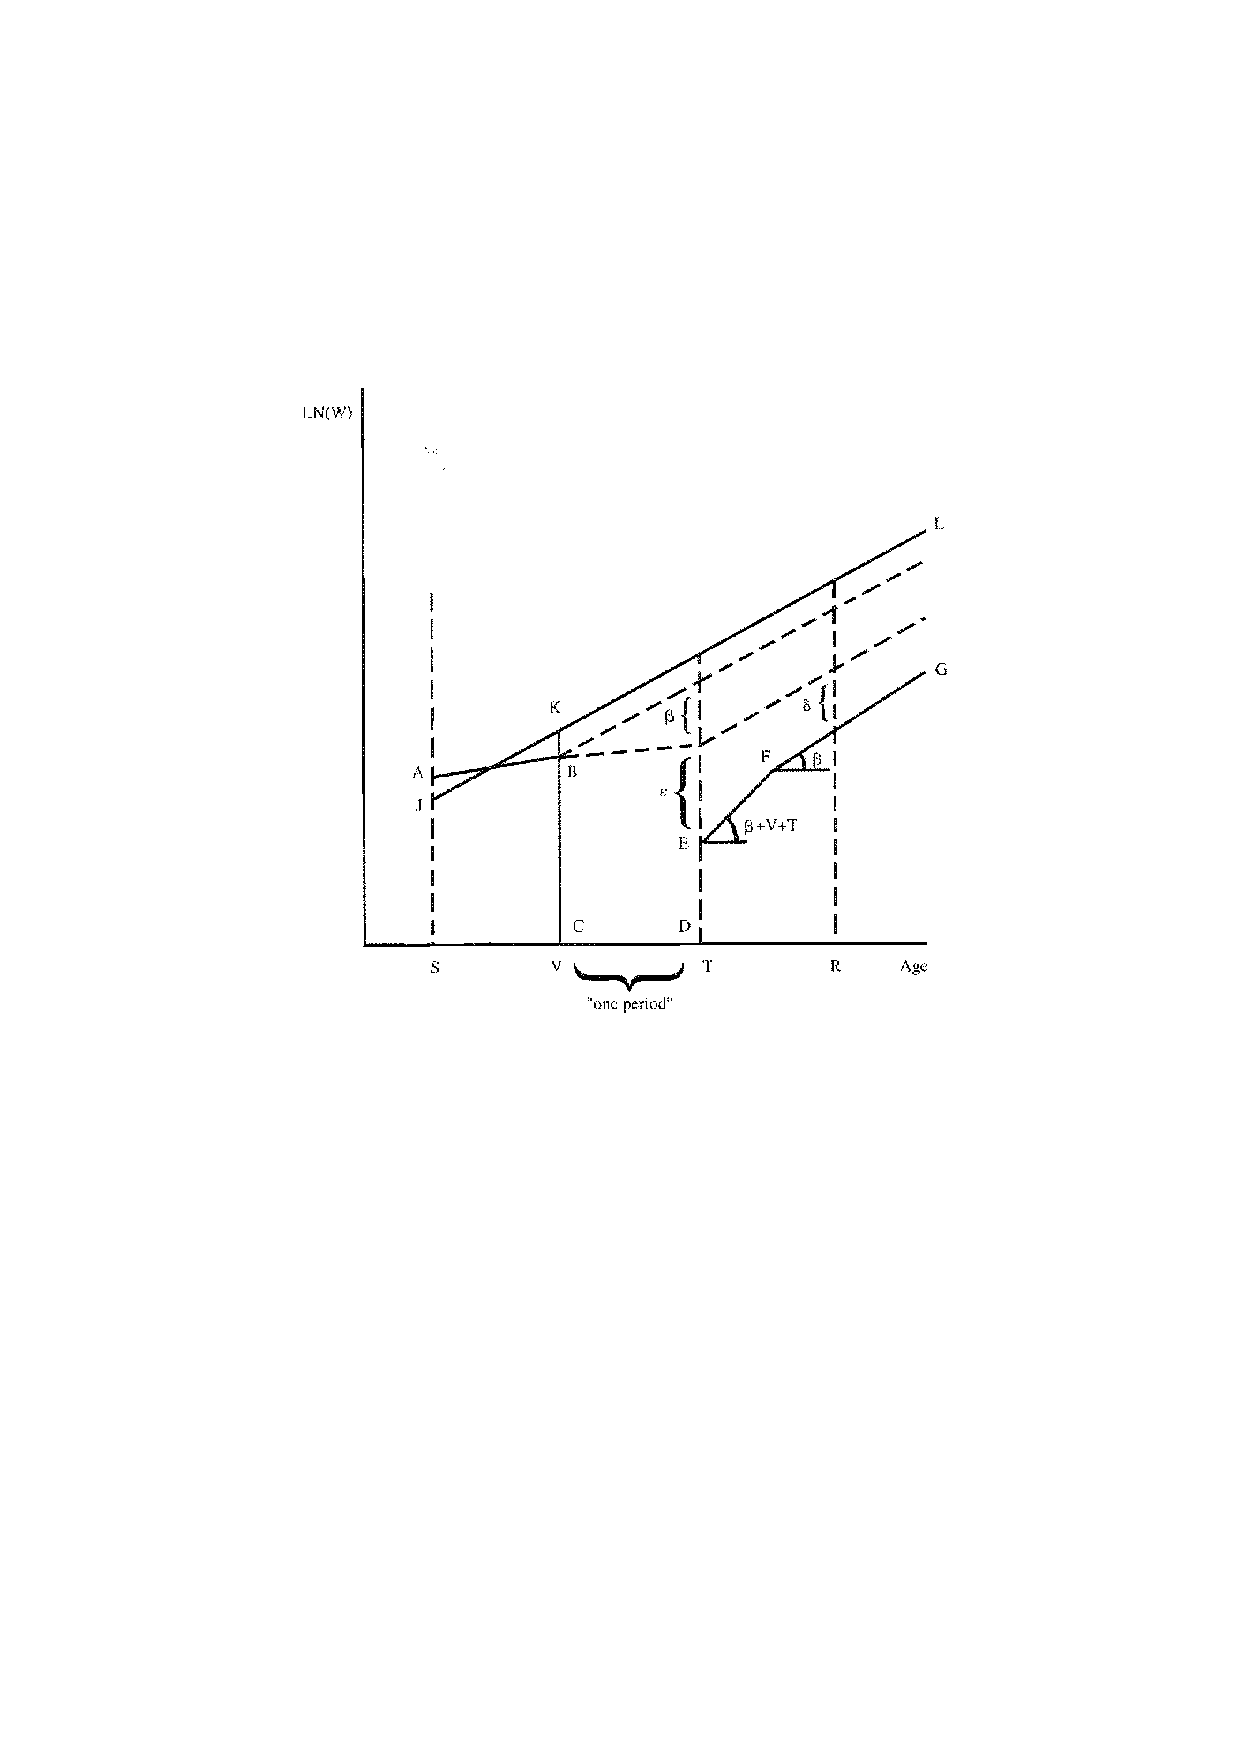
\includegraphics[width=12cm]{age_earn.pdf}
      \caption{De Grip, p. 4: "Age-earning Profile in Case of Career Interruption" see also section~\ref{sec:mincer}}
      \label{age_earn}
    \end{figure}

    \item \textbf{Economic Skills Obsolescence}\\
    However, skills can also become obsolete when new developments in society make them unnecessary (such as technical progress),
    or when a sector of the industry is shifted elsewhere (as for example production is shifted to China, etc.), or if the skills
    are firm-specific and an employee changes jobs. These factors fall into the category of \textbf{Economic} skills
    obsolescence. Given the skill-biased technical change that takes place at an accelerated pace, this type can be regarded
    as highly relevant with respect to western economies.\\
    The notion that knowledge that has been acquired in school becomes irrelevant at an increasing speed is also shown in 
    figure~\ref{earn_exp}. This figure shows the relationship between experience and earnings for different vintages of schooling.
    (Respectively for individuals that had eight, 12, and 16 years of schooling). We can see that there is a "tipping point" at
    which the relationship turns negative (probably due to economic skills obsolescence). The resulting "skills-upgrading" is 
    strongest in computer intensive industries.

      \begin{figure}[htb]
        \centering
        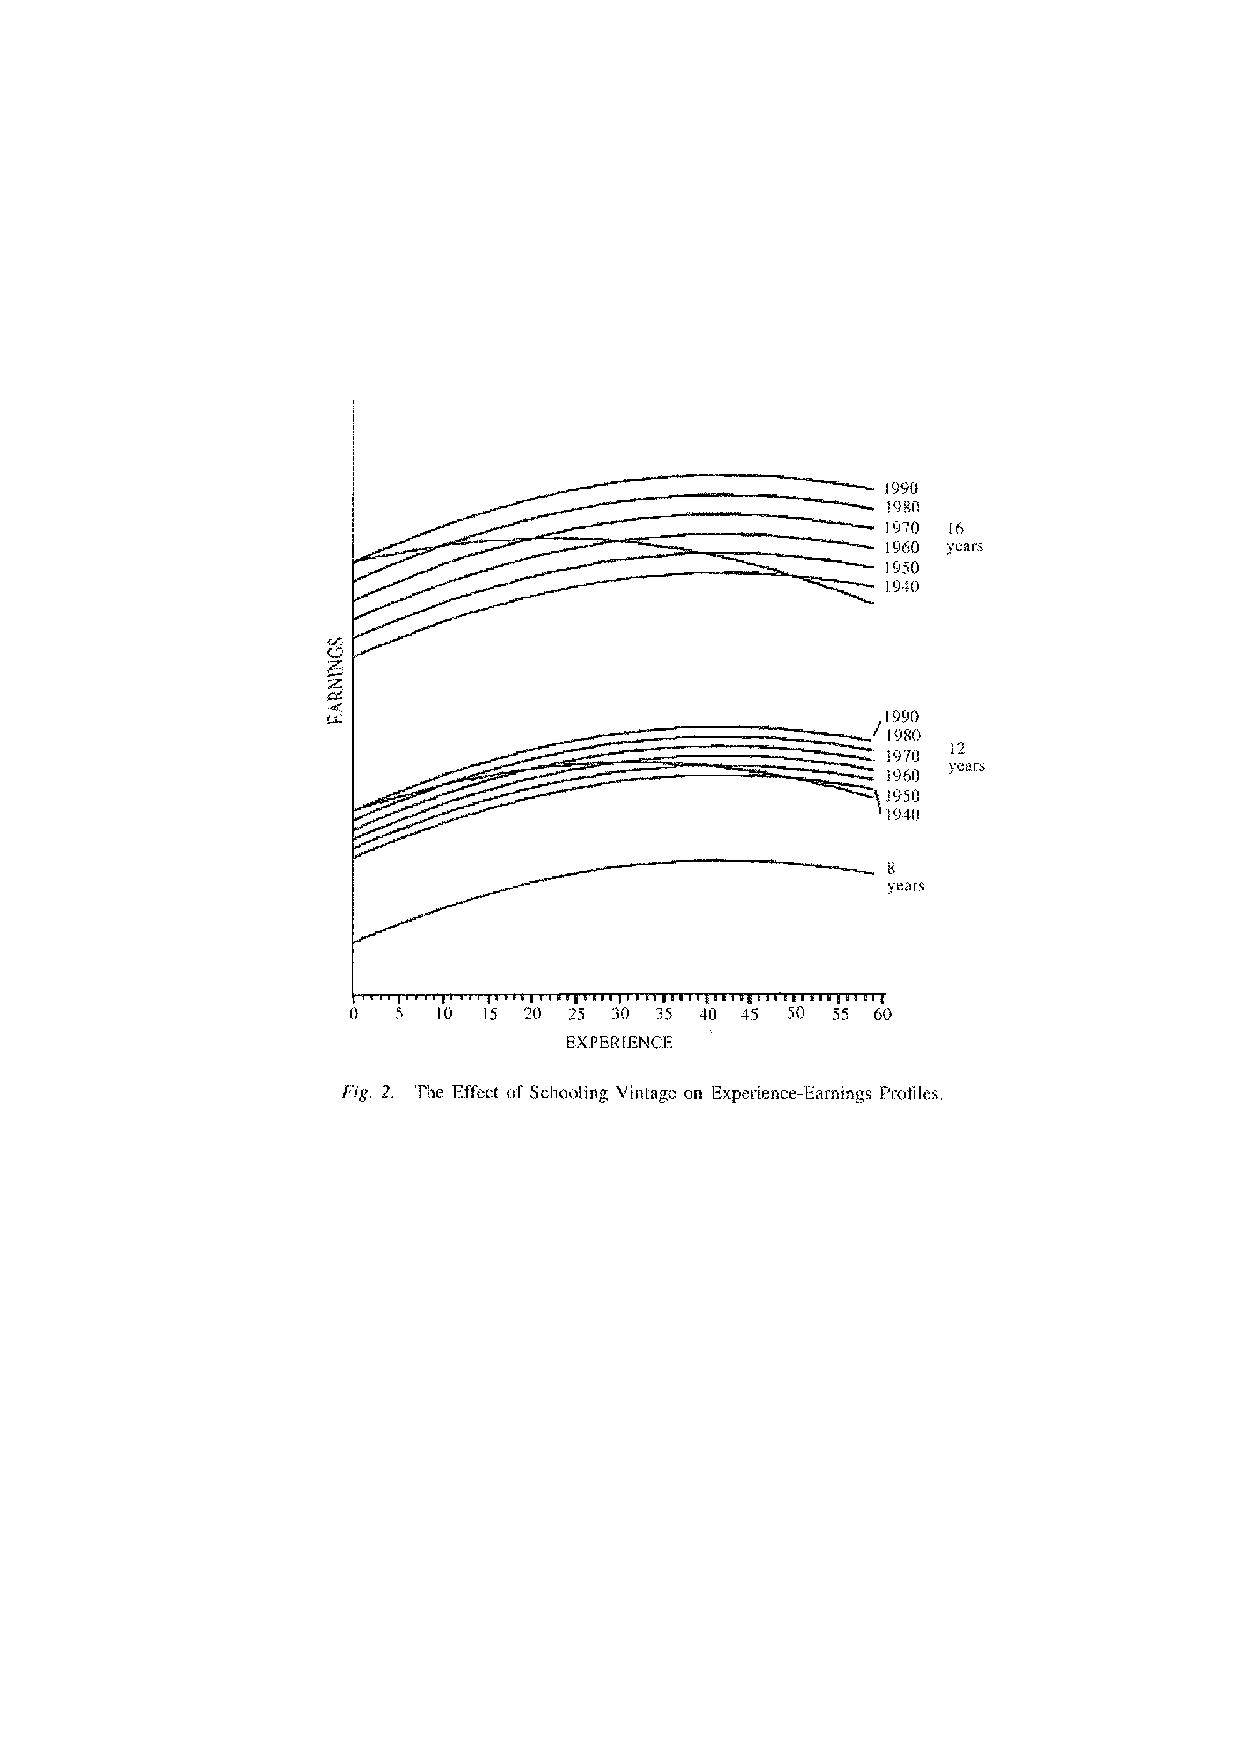
\includegraphics[width=12cm]{earn_exp.pdf}
        \caption{De Grip, p. 12}
        \label{earn_exp}
      \end{figure}


    \item \textbf{Organizational Forgetting}\\
    Here, skills obsolescence in the sense that an organization forgets
    a set of skills or practices, for example by the aggregated wear and tear or by personnel turn-over. (e.g. a fast-foot
    franchise forgets faster than a ship-building company)
  \end{itemize}


  \begin{figure}[htb]
        \centering
        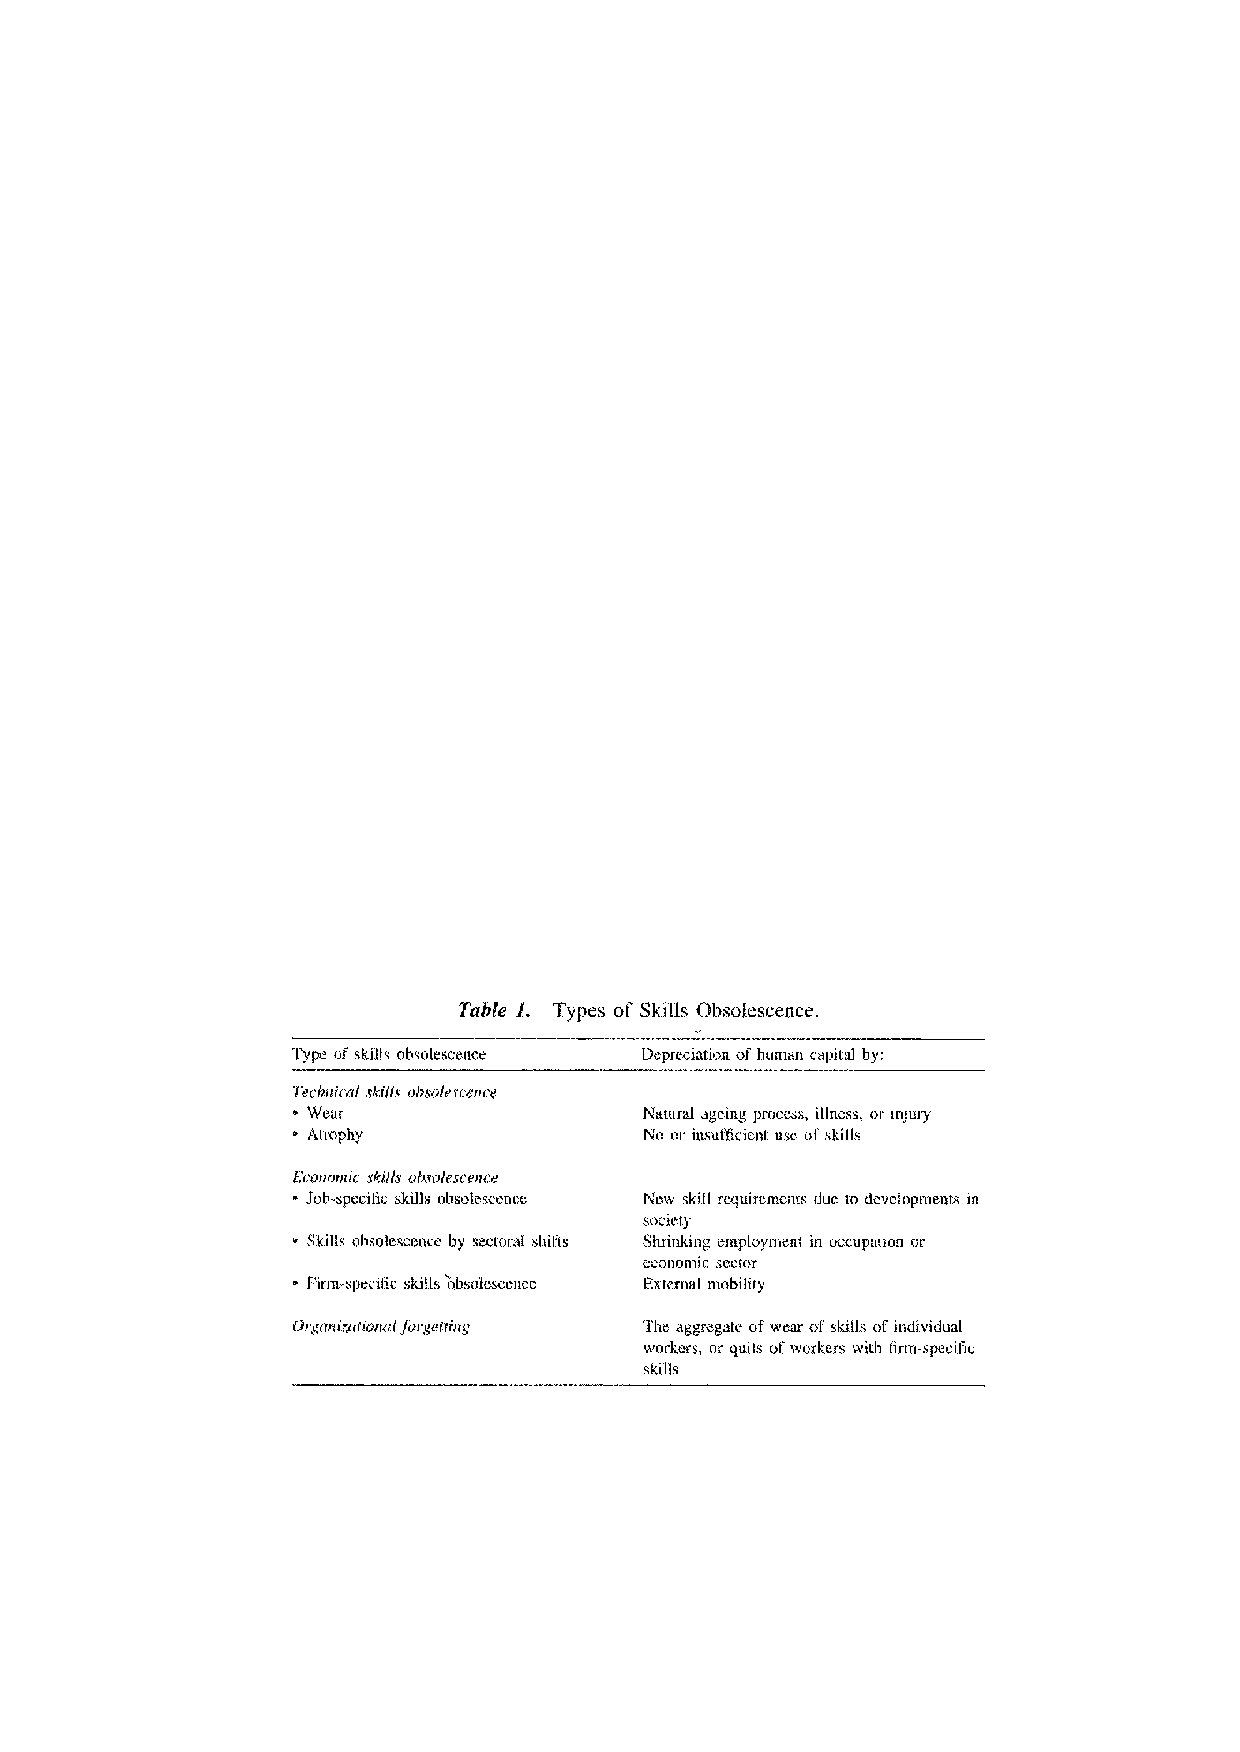
\includegraphics[width=12cm]{grip.pdf}
        \caption{De Grip, p. 4}
        \label{skill_obs}
  \end{figure}

  The authors link their findings to recent developments in the "life long learning" literature and add that the
  efforts to preserve human capital in the ageing western societies should take into account \emph{which} skills
  become obsolete more quickly. 

  \subsection{(Mincer \& Ofek, 1982) "Interrupted Work Careers: Depreciation and Restoration of Human Capital"} % (fold)
  \label{sub:mincer}
  This article discusses the wages before and after interruptions in work careers. (This links to figure~\ref{age_earn}).
  The authors show, that real wages at reentry are lower than at the point of withdrawal. This decline increases with the
  duration of the interruption. However, after reentry, there is a rapid growth of the real wage. The authors link this 
  growth to the rapid restoration of human capital (that depreciated in that sense during the interruption)\\
  It is expected the both general and specific human capital depreciate. The difference in these types of human capital
  with respect to depreciation is that losses in general capital accumulate over the time of interruption, while
  the loss of specific capital seems to be a once-for-all phenomenon.\\
  Due to the fact that the likelihood of reentry in the labor market declines with the length of the interruption, 
  it stands to reason to assume that the effects of skill depreciation are understated in the article.\\
  An effect similar to those of work interruptions can be observed in migration. Workers that come to the U.S. earn a
  lot less money at first, but then move to higher wages quickly (on average). The authors suspect that this effect
  has to do with the readaptation of human capital to another labor market. One has to note though, that the migration
  pattern in the time-frame of the analysis displays the immigration of high-skilled workers. Thus, one might also
  argue, that immigrants move to higher wages more quickly because they just invested more in human capital before
  coming to the U.S.

  % subsection mincer (end)

  \subsection{(Edin \& Gustavsson, 2005) "Time out of work and skill depreciation"} % (fold)
  \label{sub:edin}
  The authors investigate the effect of skill depreciation in the relationship between work interruptions and 
  subsequent wages. They find strong evidence for a negative relationship between work interruptions and skills.
  Furthermore, the authors find that the depreciation of information processing skills is economically significant,
  and that a full year of non-employment is equivalent to moving 5 percentiles down the skill distribution.\\
  \textbf{This article could be especially relevant since the authors use the IALS survey data}\\
  The authors mention two main strands in the literature about skill depreciation. The first strand focusses on
  women that leave their job to give birth and initially raise the child, before finally reentering the labor
  market. The second strand focusses on the role of unemployment on skill depreciation, especially with regard
  to long-term unemployment.\\
  To test empirically, the authors use the Swedish part of the IALS survey from 1994-1998. The authors first check
  that there is indeed a positive relationship between skills and wages. Then, they check the relationship between
  "time out" and skill depreciation.\\
  
  \begin{figure}[ht]
        \centering
        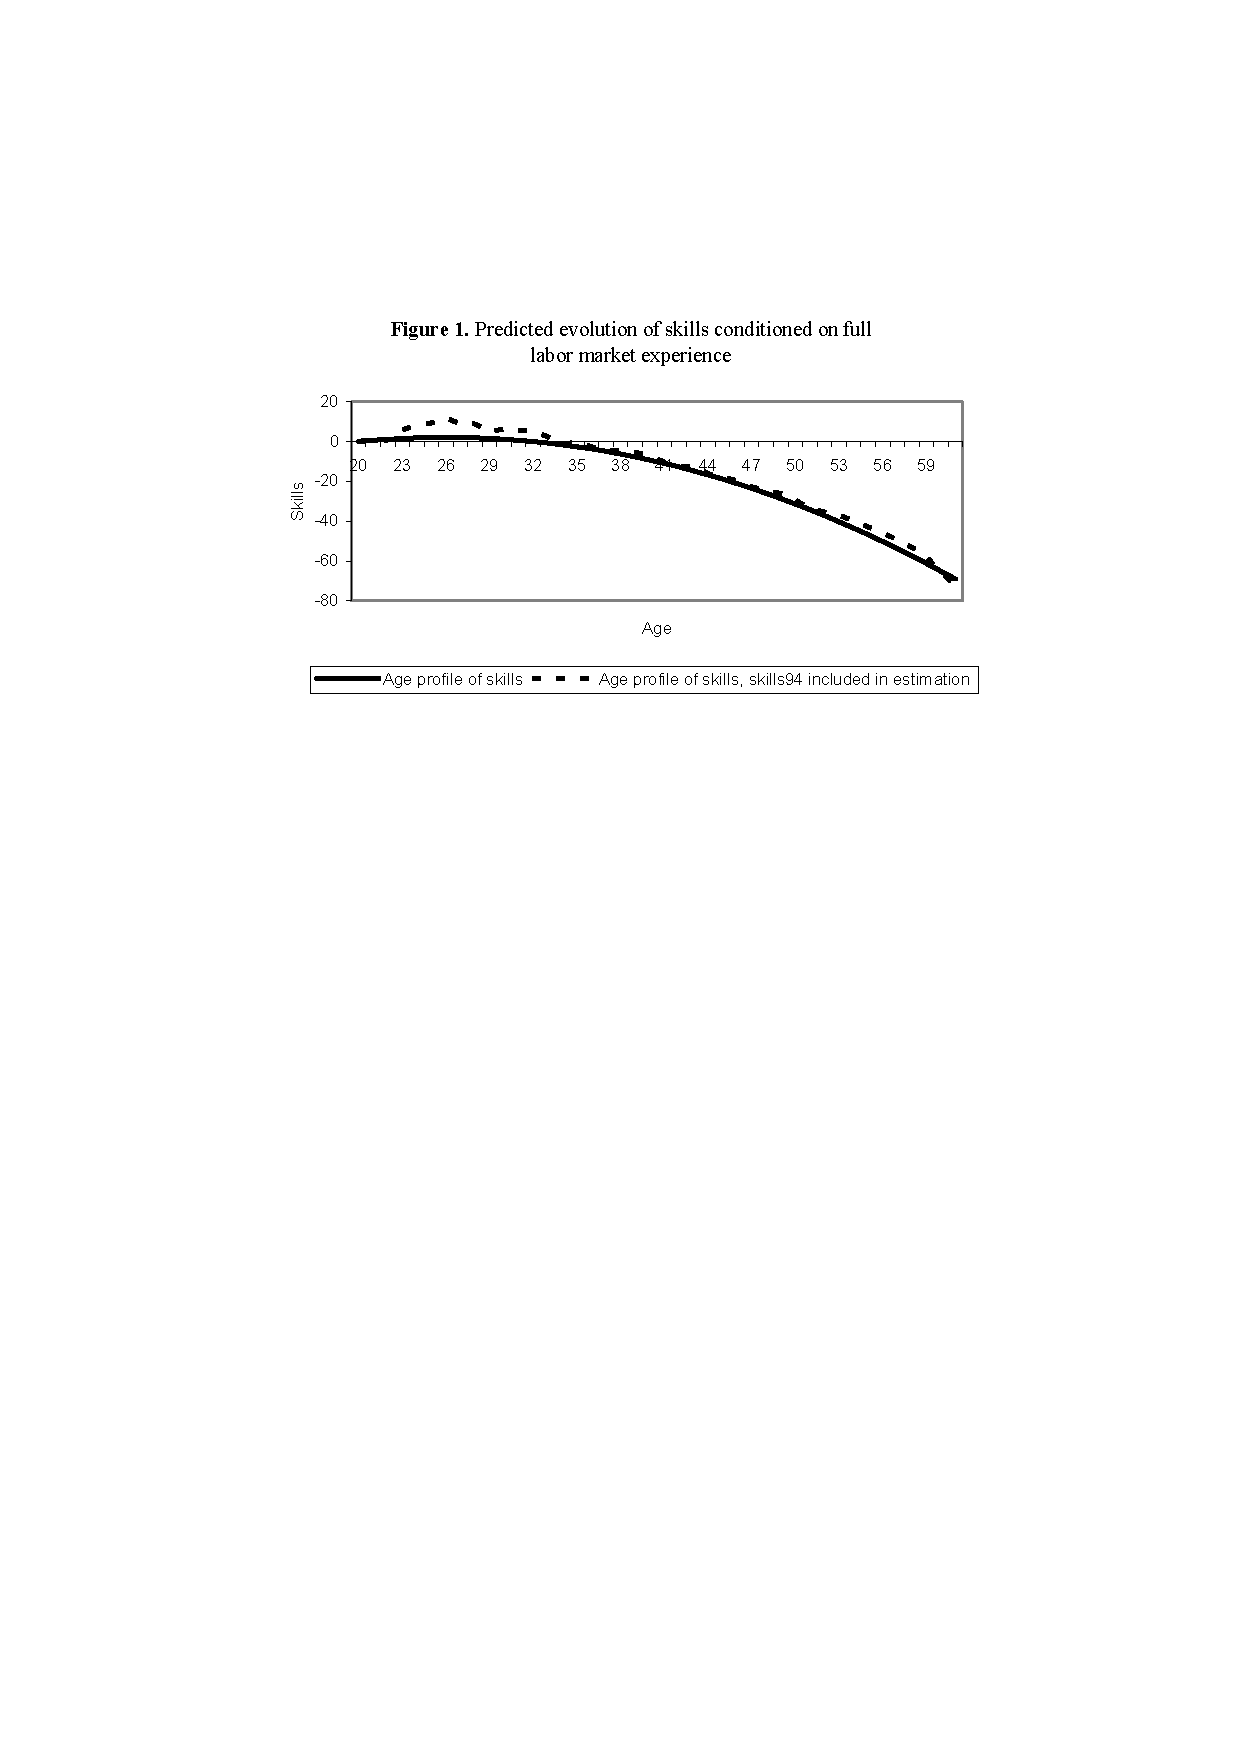
\includegraphics[width=12cm]{edin_age.pdf}
        \caption{Edin, p. 16}
        \label{edin_age}
  \end{figure}

  As a benchmark, the authors look at the general relationship of age and skills given full employment (see figure~\ref{edin_age}).
  We see again that there is a maximum at a certain age (26), after that skills decrease. In comparison to interrupted work
  careers, the relationship does indeed differ significantly. Time out of work decreases the skill level.\\
  Finally, the authors check if this lowered skill level is significant economically. Here they conclude that there is convincing
  evidence only for information processing skills. 


    \section{Meeting 10: Encouraging Human Capital Investment} % (fold)
  \label{sec:Meeting 10}
    \subsection{(Heckman, 2000) "Policies to foster human capital"}
    \label{sec:Heckman2000}

  % TODO decide whether the illustration make sense to include
  % TODO position them in the summary
  % TODO reference them in the text, explain if necessary
  \subsubsection{Illustrations to be included. …or not.}
    \begin{figure}[htb]
      \centering
      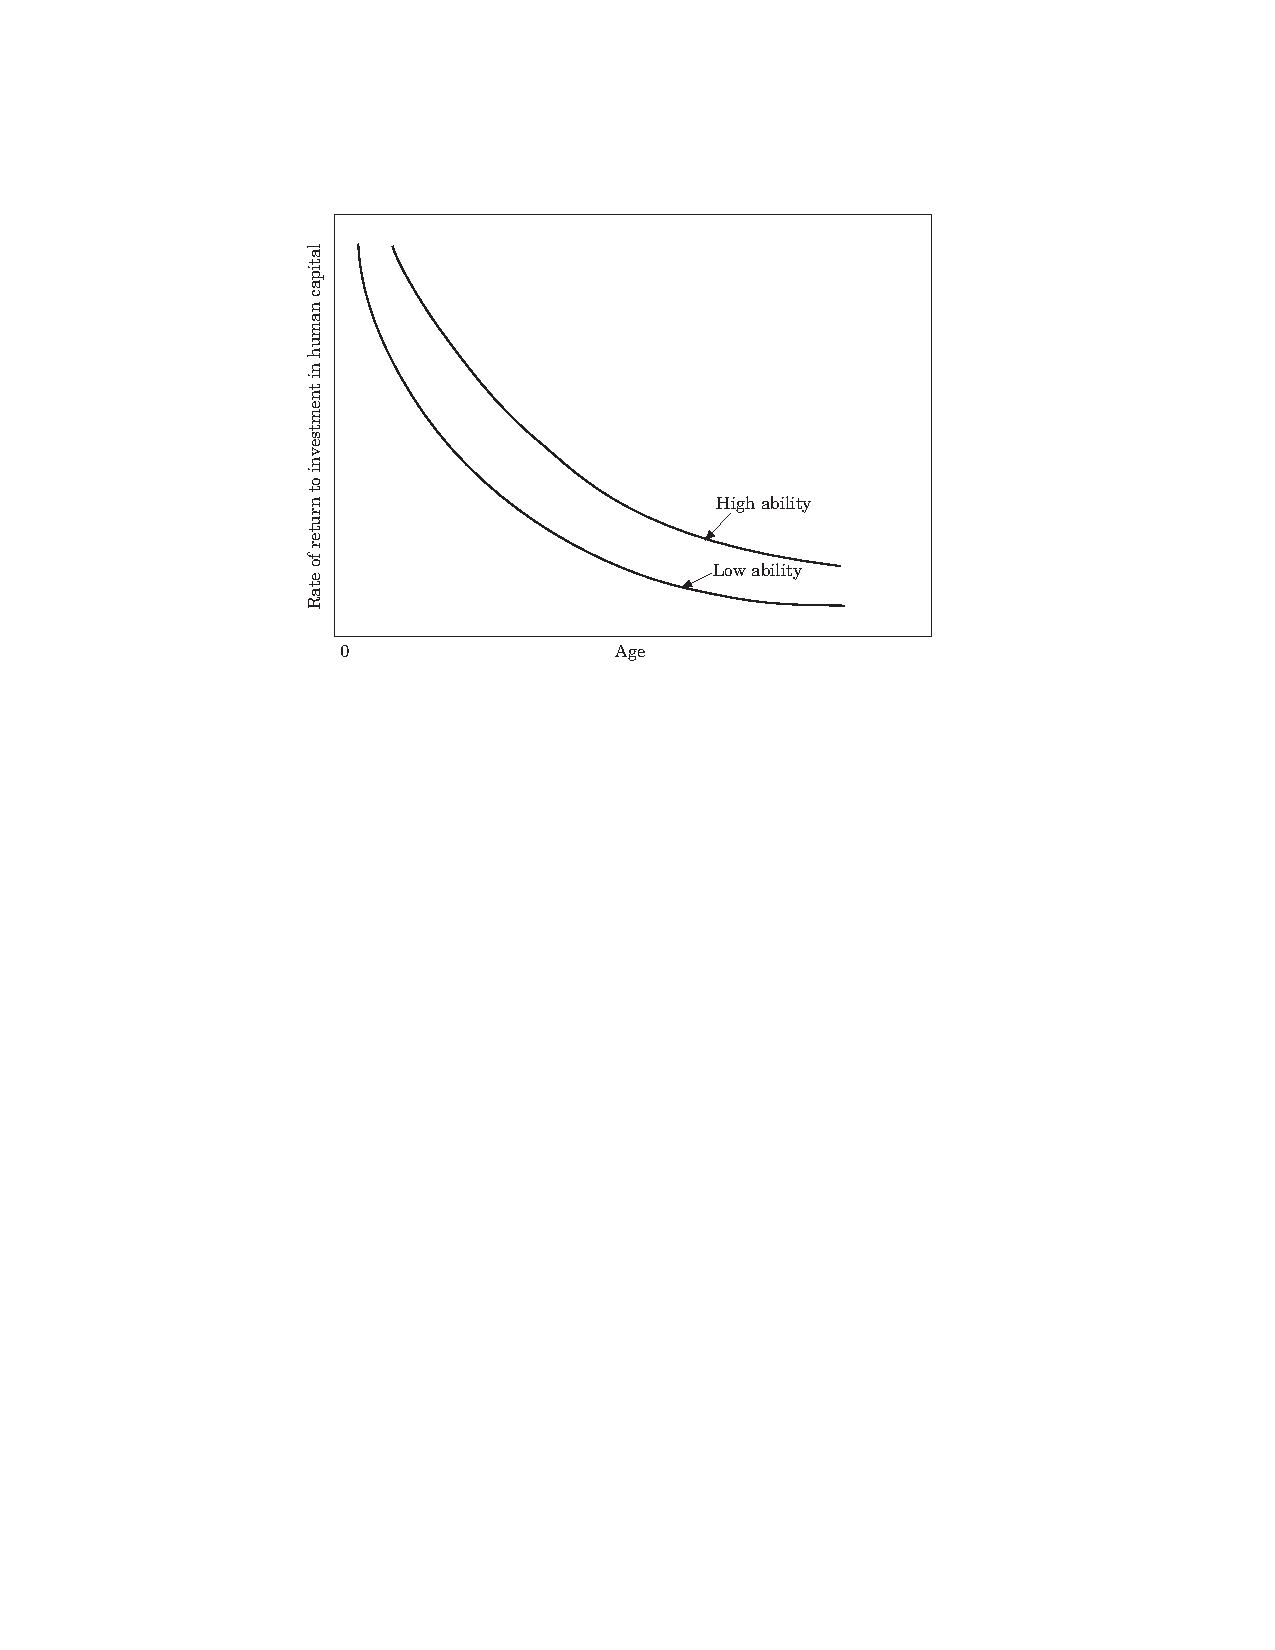
\includegraphics[width=12cm]{Meeting 10 Policies to foster human capital - Seite 7.pdf}
      \caption{Heckman, p. 7: "Rate of return to investment in human capital." see also section~\ref{sec:Heckman2000}}
      \label{fig:Heckman rateofreturnhumancapital}
    \end{figure}


    \begin{figure}[htb]
      \centering
      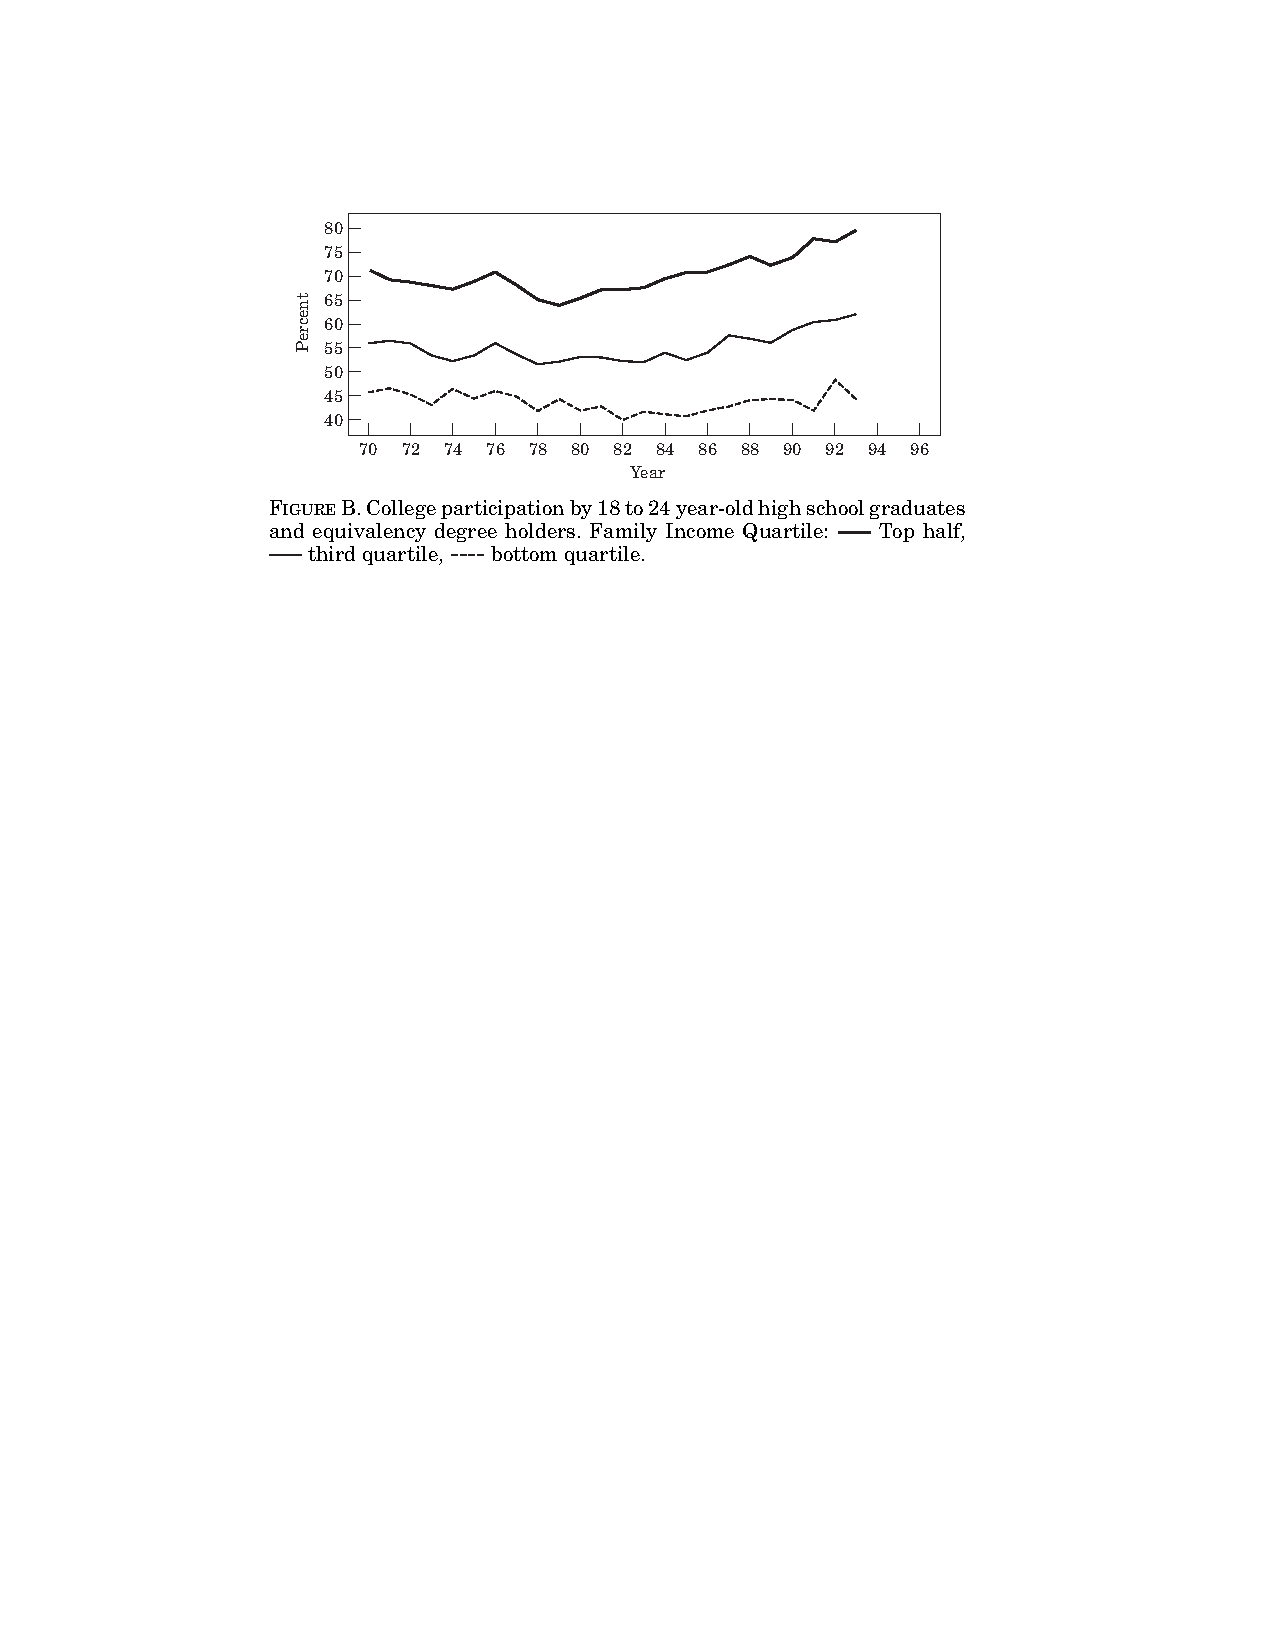
\includegraphics[width=12cm]{Meeting 10 Policies to foster human capital - Seite 11.pdf}
      \caption{Heckman, p. 11: "College participation by 18 to 24 year-old high school graduates and equivalency degree holders" see also section~\ref{sec:Heckman2000}}
      \label{fig:Heckman collegeparticipation}
    \end{figure}


    \begin{figure}[htb]
      \centering
      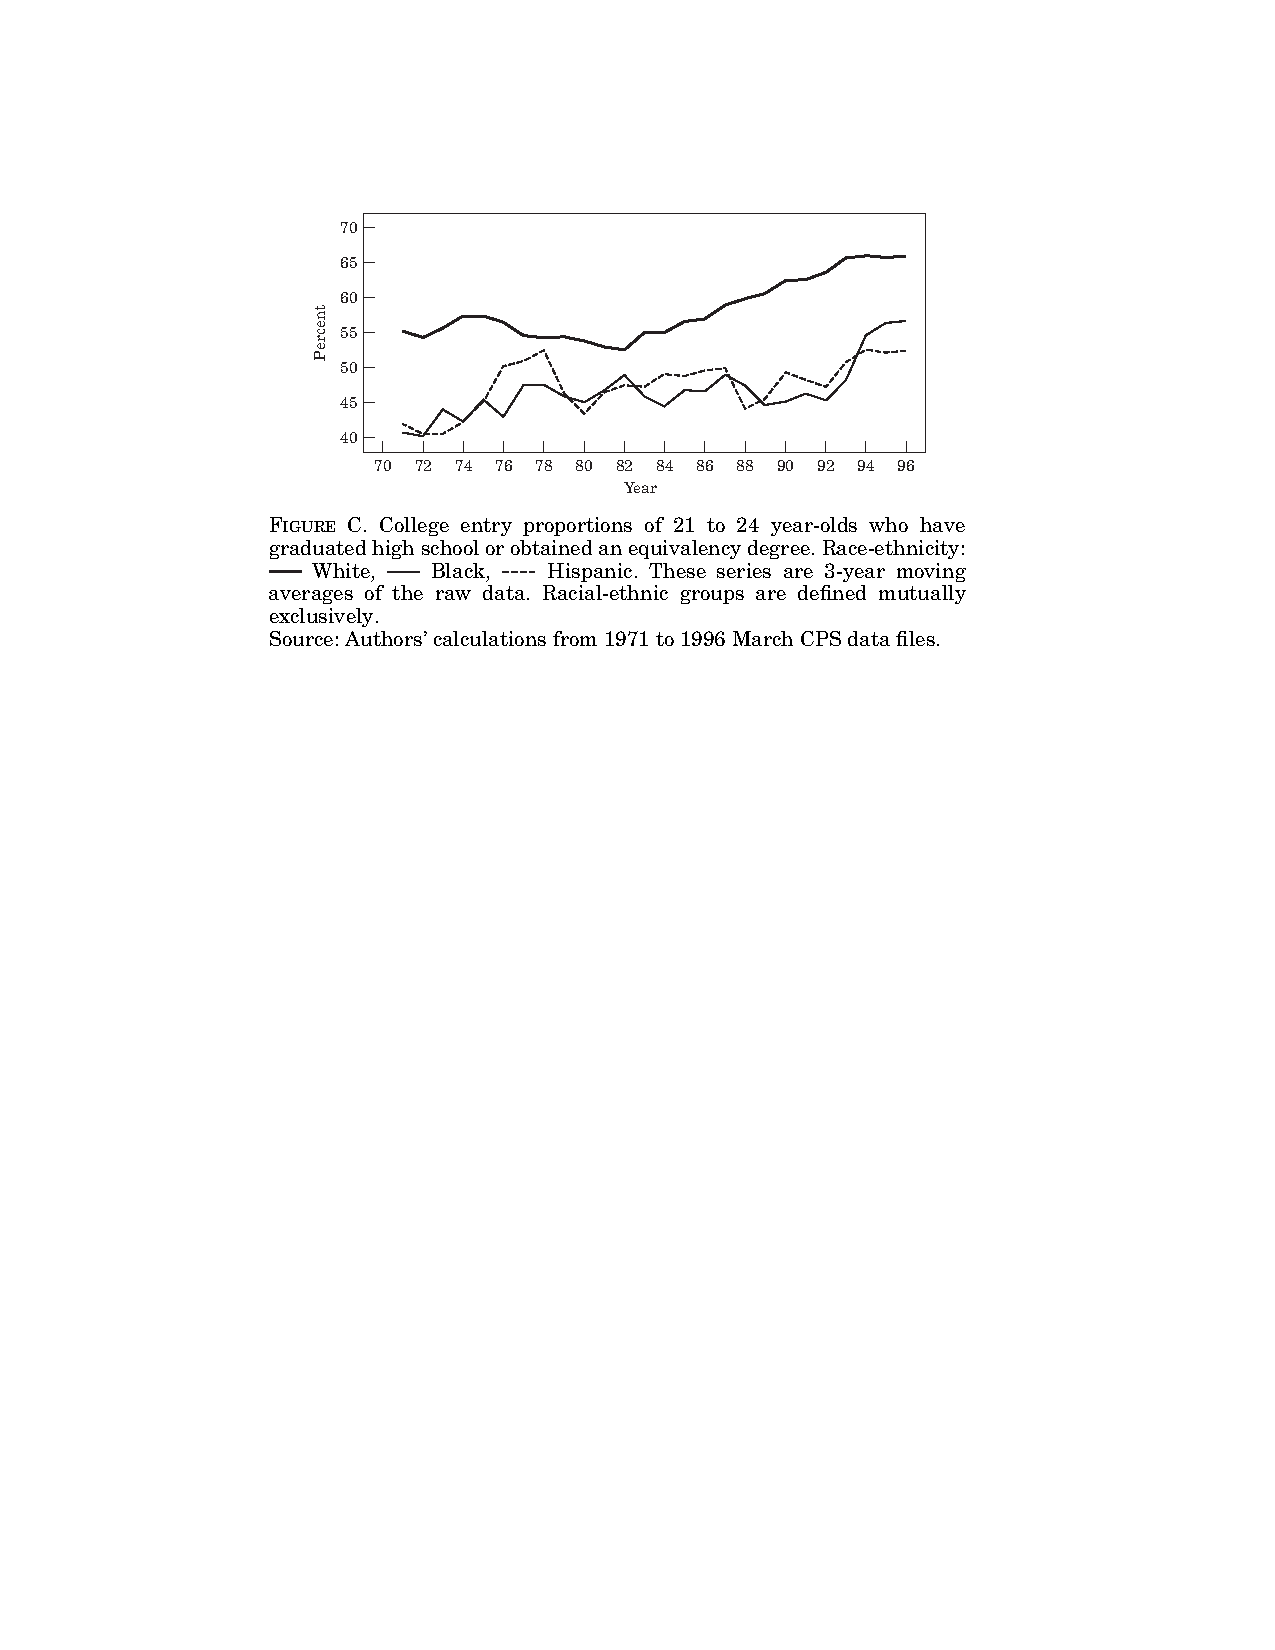
\includegraphics[width=12cm]{Meeting 10 Policies to foster human capital - Seite 14.pdf}
      \caption{Heckman, p. 14: "College entry proportions of 21 to 24 year-olds who have graduated high school or obtained an equivalency degree" see also section~\ref{sec:Heckman2000}}
      \label{fig:Heckman collegeentry}
    \end{figure}


    \begin{figure}[htb]
      \centering
      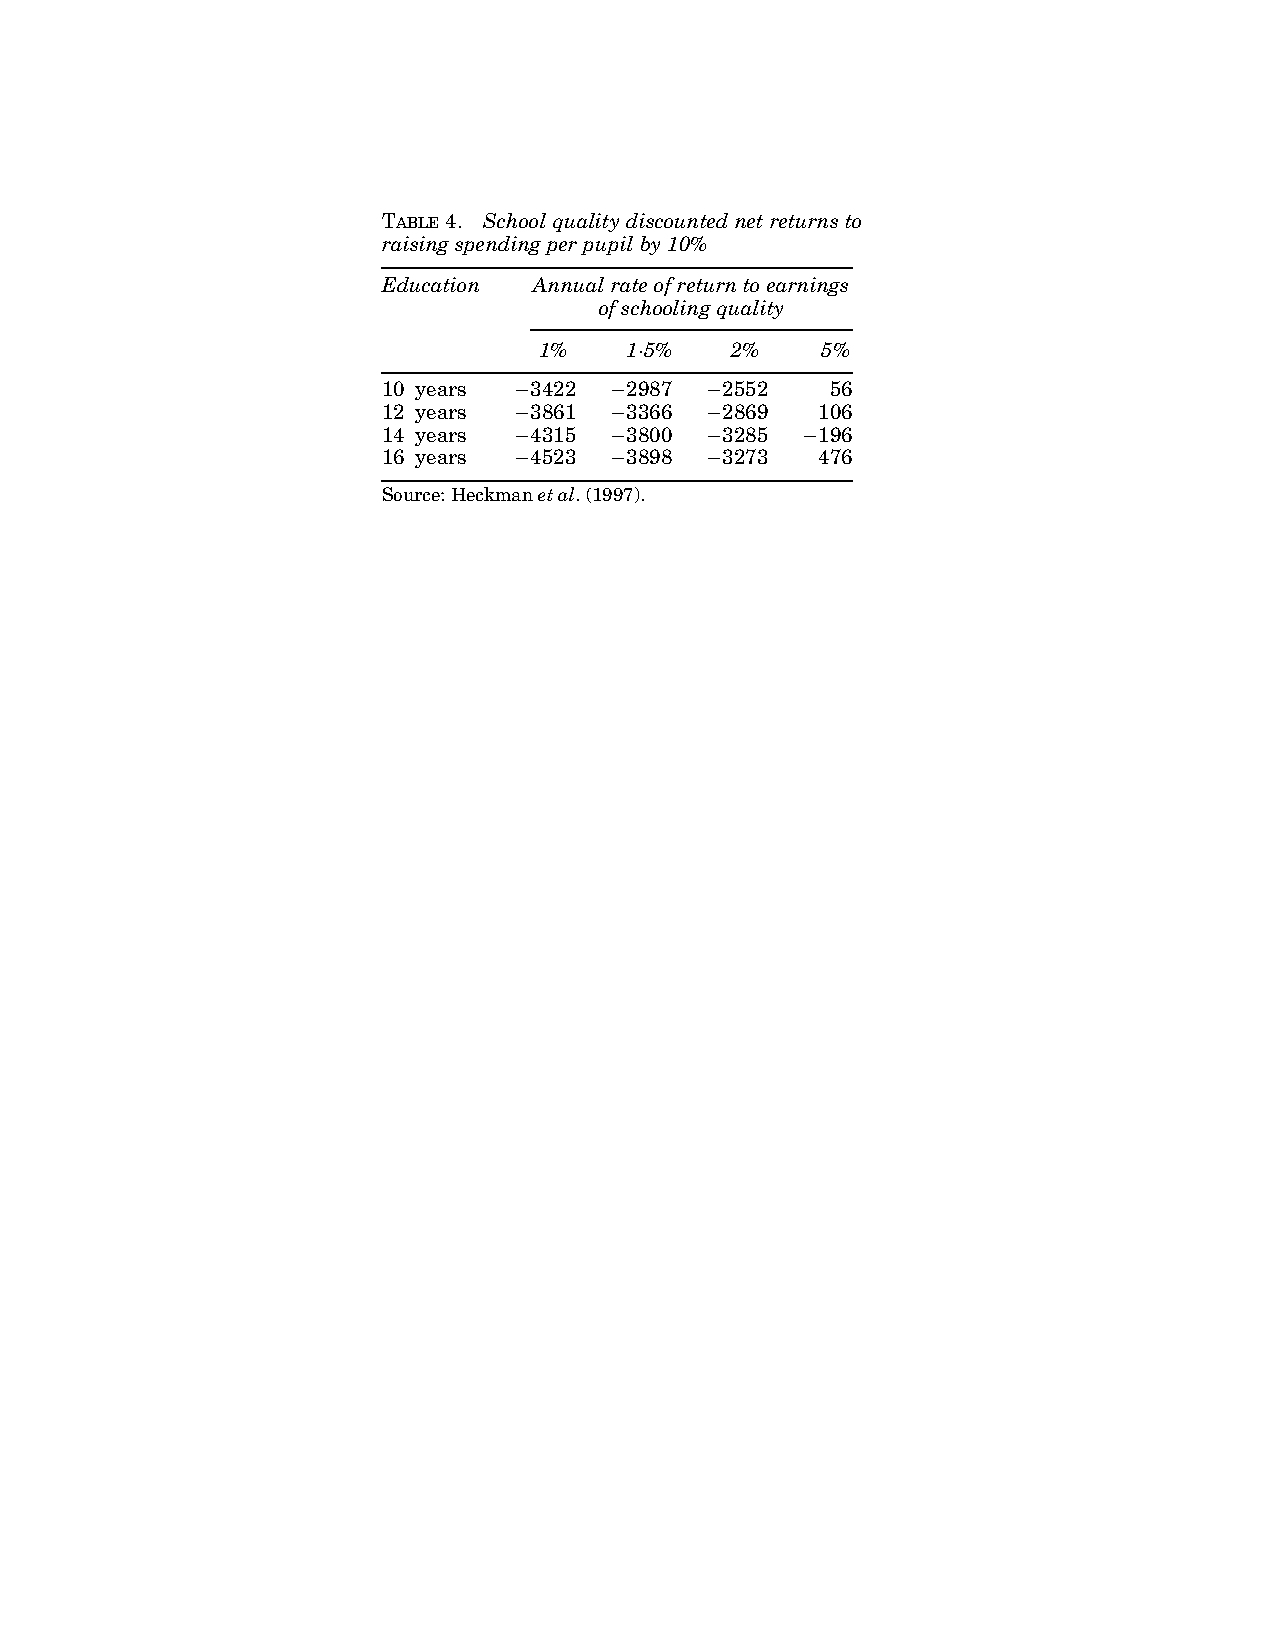
\includegraphics[width=12cm]{Meeting 10 Policies to foster human capital - Seite 20.pdf}
      \caption{Heckman, p. 20: "School quality discounted net returns to raising spending per pupil by 10\%" see also section~\ref{sec:Heckman2000}}
      \label{fig:Heckman schoolquality}
    \end{figure}


    \begin{figure}[htb]
      \centering
      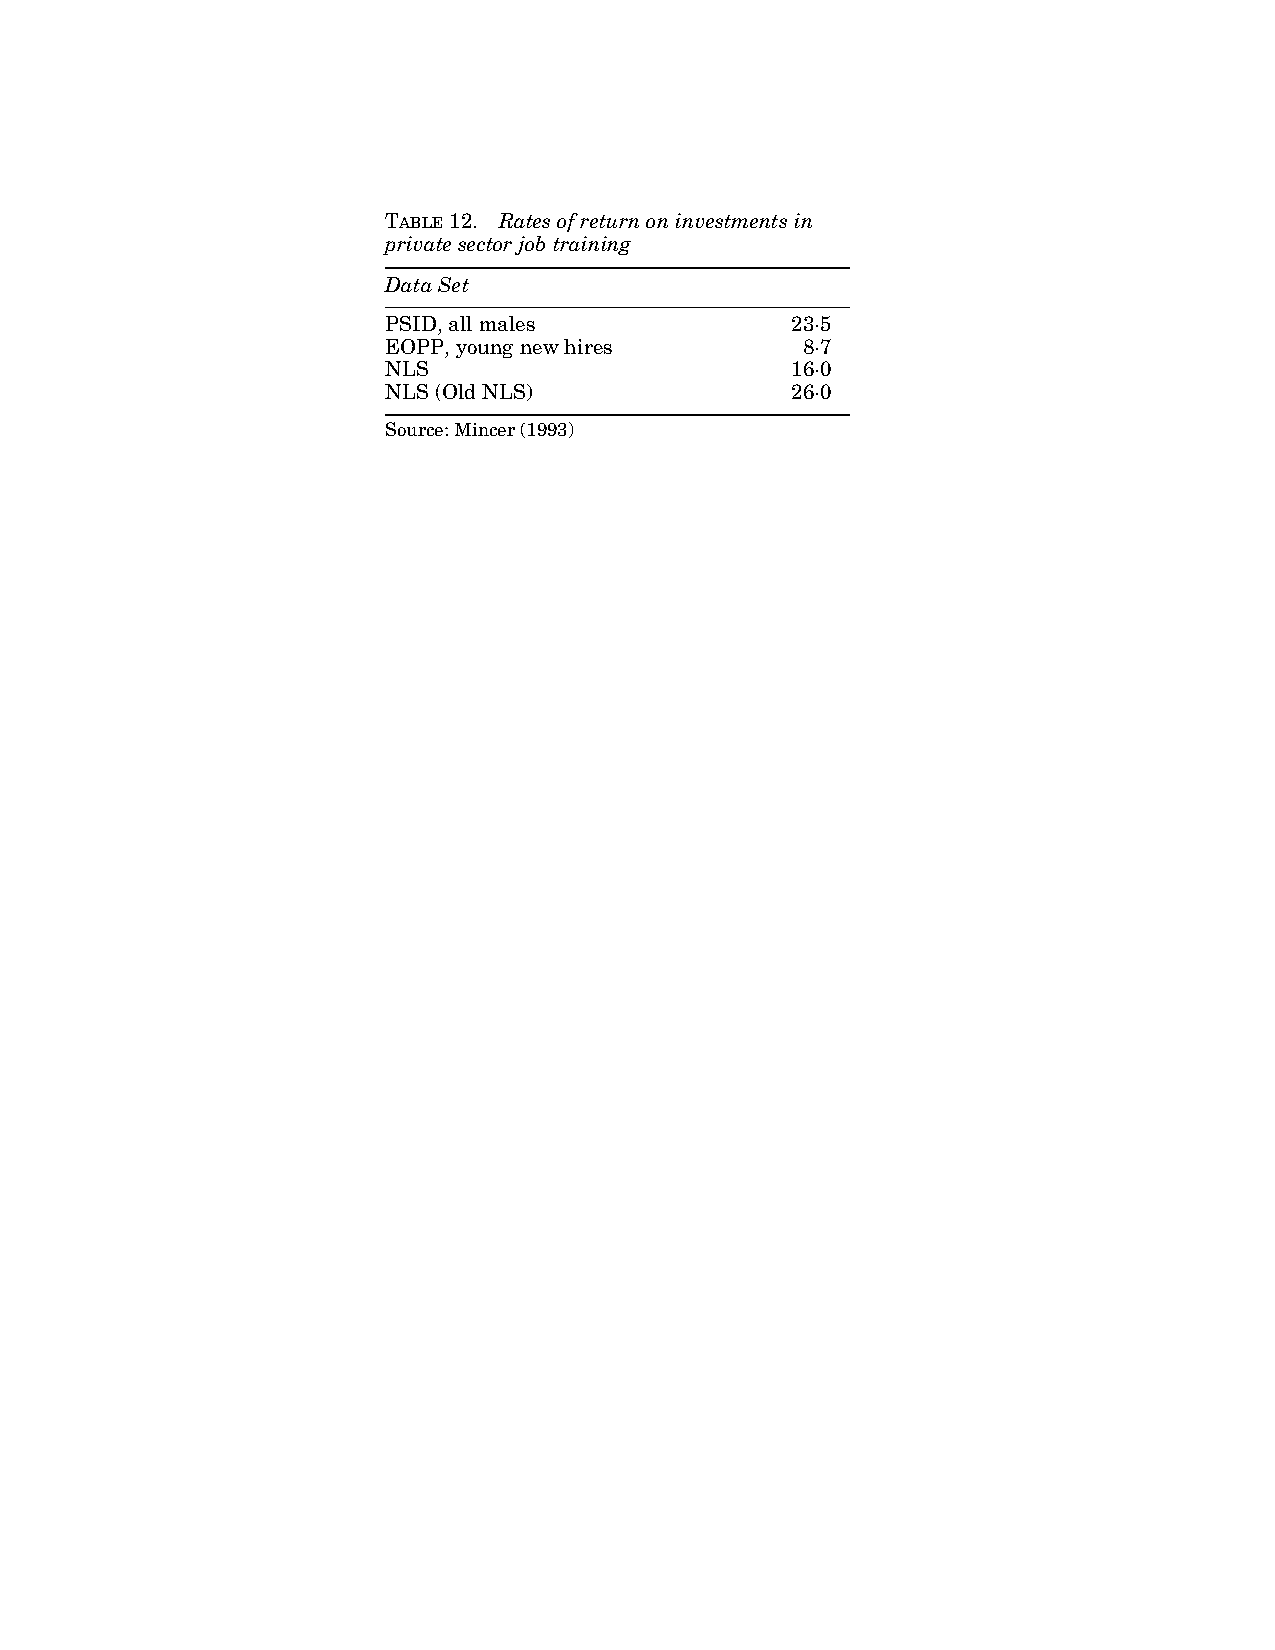
\includegraphics[width=12cm]{Meeting 10 Policies to foster human capital - Seite 37.pdf}
      \caption{Heckman, p. 37: "Rates of return on investments in private sector job training" see also section~\ref{sec:Heckman2000}}
      \label{fig:Heckman privatesectorjobtraining}
    \end{figure}


      \subsubsection{Approach}
        The paper considers the sources of skill formation in current economies and the importance of cognitive and non-cognitive skills in producing economics and social success as well. Also academic institutions, families and firms are examined as sources of learning.
      \subsubsection{Findings}
        Skills beget skills. Early investments into learning pay off much more than later investments. Non-cognitive skills and motivation are important determinants of success, much more than is usually recognized. Non-cognitive skills can be improved more successfully and at later ages than basic cognitive skills. Methods currently used to evaluate educational interventions mostly ignore these non-cognitive skills and therefore understate the benefits of early intervention programmes and mentoring and teenage motivation programmes. American society under-invests in the very young and over-invests in mature adults with low skills.

Learning begets learning: Significant improvements in the skill levels are unlikely without substantial improvements in the arrangements that foster early learning. Learning is most effective when it begins at a young age. Government interventions at an early age that mend the harm done by dysfunctional families have proven to be highly effective. This early learning is more effective for two reasons:
        \begin{itemize}
          \item younger persons have a longer horizon over which to recoup the fruits of their investments
          \item skill begets skill
        \end{itemize}
      Adults past a certain age and below a certain skill level obtain poor returns to skill investment. Reallocation of funds from investment in the old and unskilled to the young and more trainable produce more favourable outcomes in the long run. Private training programmes have two advantages:
      \begin{itemize}
        \item they can train workers who are likely to benefit
        \item they can tailor their training programmes to market needs
      \end{itemize}
      By encouraging work rather than unemployment and crime, wage subsidies for the older generation in light of a technological shift may also provide social benefits that extend beyond individual increases in earnings. Governments subsidize higher education, and those subsidies benefit both unskilled and skilled workers. Evidence that borrowing constraints are important deterrents to college attendance is very weak though. Lower family income levels are associated with less productive family and neighbourhood environments, as well as lower motivation and ability by prospective students. Available evidence suggests that additional spending on public school quality would be inefficient. Reforms in the administrative structure of education and infusion of incentives and competition are far more likely to be effective.

      Reforms to eliminate progressivity in the tax system will have only small effects on human capital accumulation. Far more important for wage growth and economic efficiency are reforms in the taxation of capital. Promoting capital formation raises the real wages of skilled and unskilled workers with only slight effects on inequality in earnings.

    \subsection{(Jenkins \& Vignoles, 2003) "The determinants and labour market effects of lifelong learning"}
      \subsubsection{Approach}
      Uses rich longitudinal panel data to find key factors that determine whether someone undertakes lifelong learning and models the effect of the different qualifications on wages and the likelihood of being employed.

      \subsubsection{Findings}
      Similar to Heckman, learning begets learning. Undertaking one episode of lifelong learning also increased the probability of undertaking more lifelong learning. Acquiring qualifications at school increases the likelihood of undertaking lifelong learning. There is little evidence of positive wage effects. Some specific types of lifelong learning do appear to boost the wages of the least qualified workers. Robust evidence that men who left school with only low-level qualifications, who then acquired degrees via lifelong learning, earned more than their peers. Stronger evidence of employment effects from lifelong learning, associated with a higher probability of being in the labour market. One possible explanation for the results is that qualifications provide a signal to employers of a person’s ability to do the job. Perhaps acquiring qualifications late in life does not send the same signal to employers as acquiring them early on.

  % section Meeting 10 (end)

  \appendix
\section{Glossary} % (fold)
  \label{sec:Glossary}
  \subsection{Instrumental Variables (IV)} % (fold)
  \label{sub:IV}
  In statistics, econometrics, epidemiology and related disciplines,
  the method of instrumental variables (IV) is used to estimate
  causal relationships when controlled experiments are not feasible.
  Statistically, IV methods allow consistent estimation when the
  explanatory variables (covariates) are correlated with the error terms.
  Such correlation may occur when the dependent variable causes at least
  one of the covariates ("reverse" causation), when there are relevant
  explanatory variables which are omitted from the model, or when the
  covariates are subject to measurement error. In this situation, ordinary
  linear regression generally produces biased and inconsistent estimates.
  However, if an instrument is available, consistent estimates may still
  be obtained. An instrument is a variable that does not itself belong
  in the explanatory equation and is correlated with the endogenous
  explanatory variables, conditional on the other covariates. 

  In linear models, there are two main requirements for using an IV:
  \begin{itemize}
    \item The instrument must be correlated with the endogenous explanatory variables, conditional on the other covariates.
    \item The instrument cannot be correlated with the error term in the explanatory equation, that is, the instrument cannot suffer from the same problem as the original predicting variable.
  \end{itemize}
  \footnotesize{Source: Wikipedia}
  % subsection IV (end)
  % section Glossary (end)
  \end{document}
